

%\frame{
%  \frametitle{Misure di precisione nel Modello Standard e nel settore dell'Higgs}
%}


%\setbeamertemplate{background canvas} {
%\begin{figure}
%\centering
%\includegraphics[scale=0.68]{logoHPD.jpg}
%\end{figure}
%}

\frame{\frametitle{Nuove particelle scoperte a LHC - test QCD}
\begin{columns}[c]
\begin{column}{1.15\linewidth}
\centering
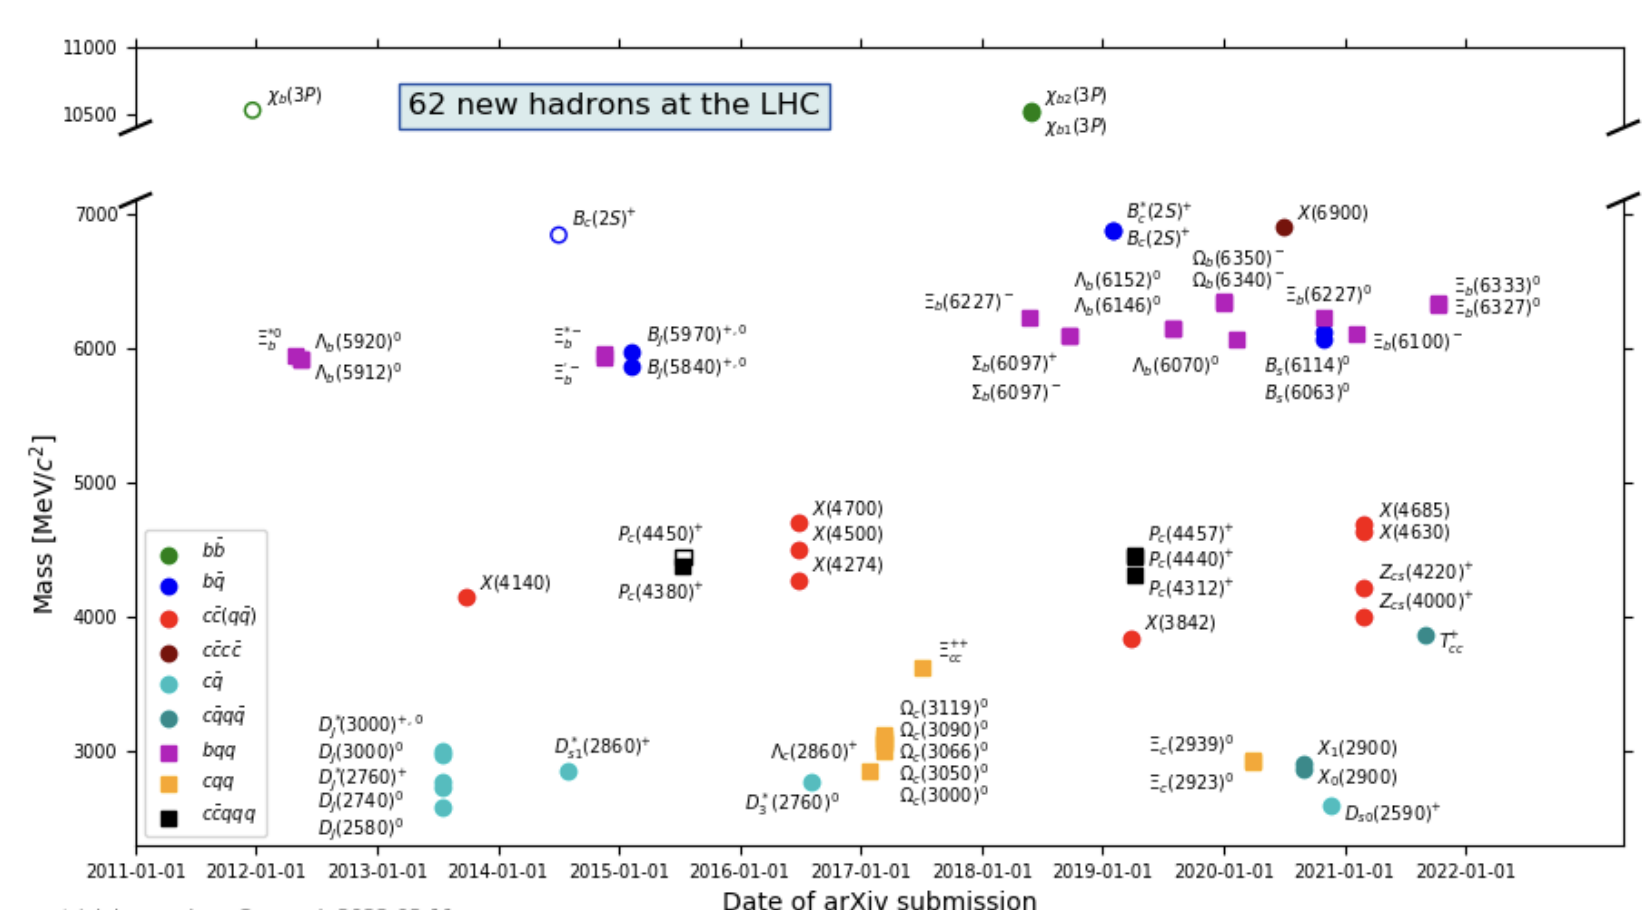
\includegraphics[scale=0.35]{figs/particlediscoveryatLHC.png}
\end{column}
\end{columns}
\begin{columns}[c]
\begin{column}{0.7\linewidth}
\begin{itemize}
\scriptsize
\item 62 nuove adroni scoperti a LHC
\item Test di modelli di QCD (Heavy Quark Effective Theory, ...)
\item Tra questi adroni esotici: tetraquark, pentaquark! 
\end{itemize}
\end{column}
\begin{column}{0.45\linewidth}
\centering
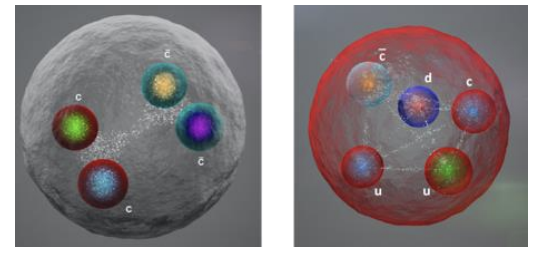
\includegraphics[scale=0.35]{figs/tetraquarkpentaquark.png}
\end{column}
\end{columns}
}

\frame{\frametitle{Settore del sapore: Flavour Changing Neutral Current (FCNC)}

\begin{columns}[c]
\begin{column}{1.15\linewidth}
\begin{itemize}
\scriptsize
\item Modelli di Nuova Fisica: esistenza di nuove particelle
\item Molti processi rari e soppressi
\item Sensibili a Nuova Fisica a scale molto più elevate attraverso
  effetti nei loop di nuove particelle BSM
\item Particolarmente interessanti: correnti neutre con cambiamento di
  sapore (FCNC)
    \end{itemize}
\centering
\scriptsize
$B_s^0 - \bar{B}_s^0$ mixing \quad \quad \quad \quad \quad \quad \quad \quad \quad \quad $B^0 \rightarrow K^{*0} \mu^+ \mu^-$ \\
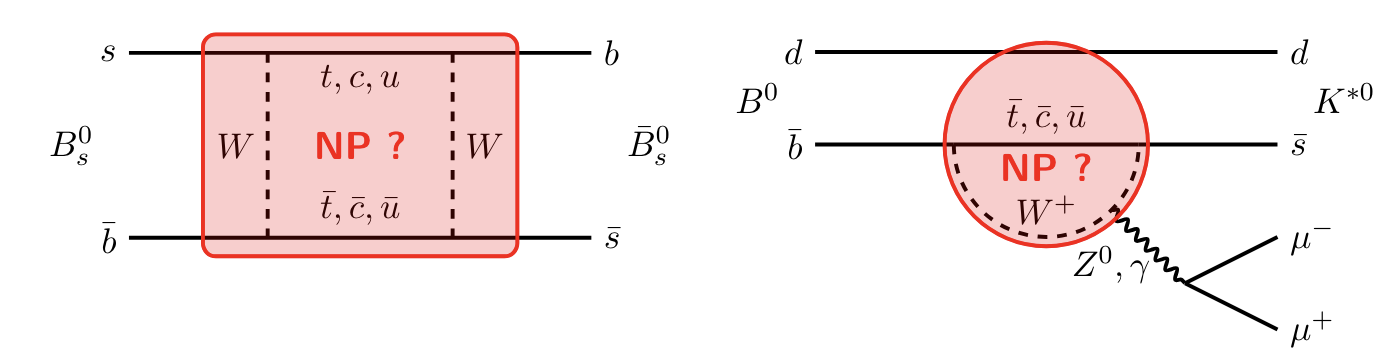
\includegraphics[scale=0.5]{figs/FCNC.png}\\
\begin{itemize}
\item Possibili nuove fasi di violazione CP, effetti su branching
  fraction e distribuzioni angolari
\end{itemize}
\end{column}
\end{columns}
}




\frame{\frametitle{Settore del Sapore}
\begin{columns}[c]
\begin{column}{1.15\linewidth}
\begin{itemize}
\scriptsize
\item Sono molte le domande aperte legate esplicitamente al settore del sapore del
  Modello Standard
\item Perch\`e ci sono 3 generazioni di quark?
\item Perch\`e la matrice CKM \`e praticamente diagonale mentre la
  matrice PMNS no?
\item Violazione di CP?
\end{itemize}
\end{column}
\end{columns}

}



%\frame{\frametitle{Violazione di CP}
%\begin{columns}[c]
%\begin{column}{1.15\linewidth}
%\begin{itemize}
%\scriptsize
%\item Le	condizioni di Sakharov possono verificarsi nel MS
%  in un modello di bariogenesi elettrodebole.
%\item La	non	conservazione	del numero barionico e
%  l'uscita dall'equilibrio termodinamico possono essere	avvenute
%  ad una temperatura pari alla	massa del bosone $W$, $T_{EW} \sim
%  {\mathcal O}(100)
%  \unitm{GeV}$, che	l'Universo ebbe al momento della transizione di fase	elettrodebole.	
%\item Se si considera la violazione di CP causata dal meccanismo
%  CKM non \`e sufficiente per spiegare l'asimmetria
%  materia-antimateria dell'Universo:\\
%$\Delta  = \frac{J \times P_{u} \times P_{d}}{T_{EW}^{2}}$\\
%con $P_{u} \times P_{d} = (m_{t}^{2}-m_{c}^{2}) (m_{t}^{2}-m_{u}^{2}) (m_{c}^{2}-m_{u}^{2}) (m_{b}^{2}-m_{s}^{2}) (m_{b}^{2}-m_{d}^{2}) (m_{s}^{2}-m_{d}^{2})$\\ 
%$\Delta \sim 10^{-19} \ll 10^{-10}$\\ 
%\end{itemize}
%\end{column}
%\end{columns}
%}

\frame{\frametitle{Violazione di CP oltre il MS}
\begin{columns}[c]
\begin{column}{1.0\linewidth}
\begin{itemize}
\scriptsize
\item L'asimmetria tra materia e anti-materia osservata nell'Universo
  richiede una non-conservazione di CP di entit\`a molto maggiore di
  quanto previsto dal MS nel settore dei quark.
\item Quale \`e l'origine	della violazione di CP presente
  nell'Universo in cui viviamo?
\item Che cosa ha causato l'asimmetria materia-antimateria
  nell'Universo rimane uno dei problemi attuali
\item Determinazione se la quantit\`a di CP osservata \`e
  compatibile con quella prevista dal MS
\item Per avere una grande asimmetria \`e richiesta una nuova sorgente
  di violazione di CP
\begin{itemize}
\scriptsize
\item Settore leptonico: \`e necessario studiare la violazione CP
  nelle oscillazioni dei neutrini (misura della fase $\delta$ nella
  matrice PMNS agli esperimenti long-baseline con fasci di
  neutrini agli acceleratori come T2K (Giappone) , NO$\nu$A (USA) DUNE
  (USA))
\item Settore dei quark: si cercano discrepanze tra le misure di CPV e
  le previsioni di CKM (Esperimenti LHCb (CERN) e BelleII (KEK, Giappone))
\item Settore di gauge: misure dirette o indirette sensibili alla
  presenza di nuove interazioni (dove potrebbe esserci violazione di
  CP)
\item Violazione di CP nella QCD (termine di violazione di CP
  non è stato osservato sperimentalmente, problema CP forte,
  meccanismo di Peccei-Quinn con l'introduzione di una nuova
  particella: assione)
\end{itemize}
\end{itemize}
\end{column}
\end{columns}
}







\frame{\frametitle{Settore del sapore: UT}
\begin{columns}[c]
\begin{column}{1.0\linewidth}
\centering
\scriptsize
Attuale conoscenza\\
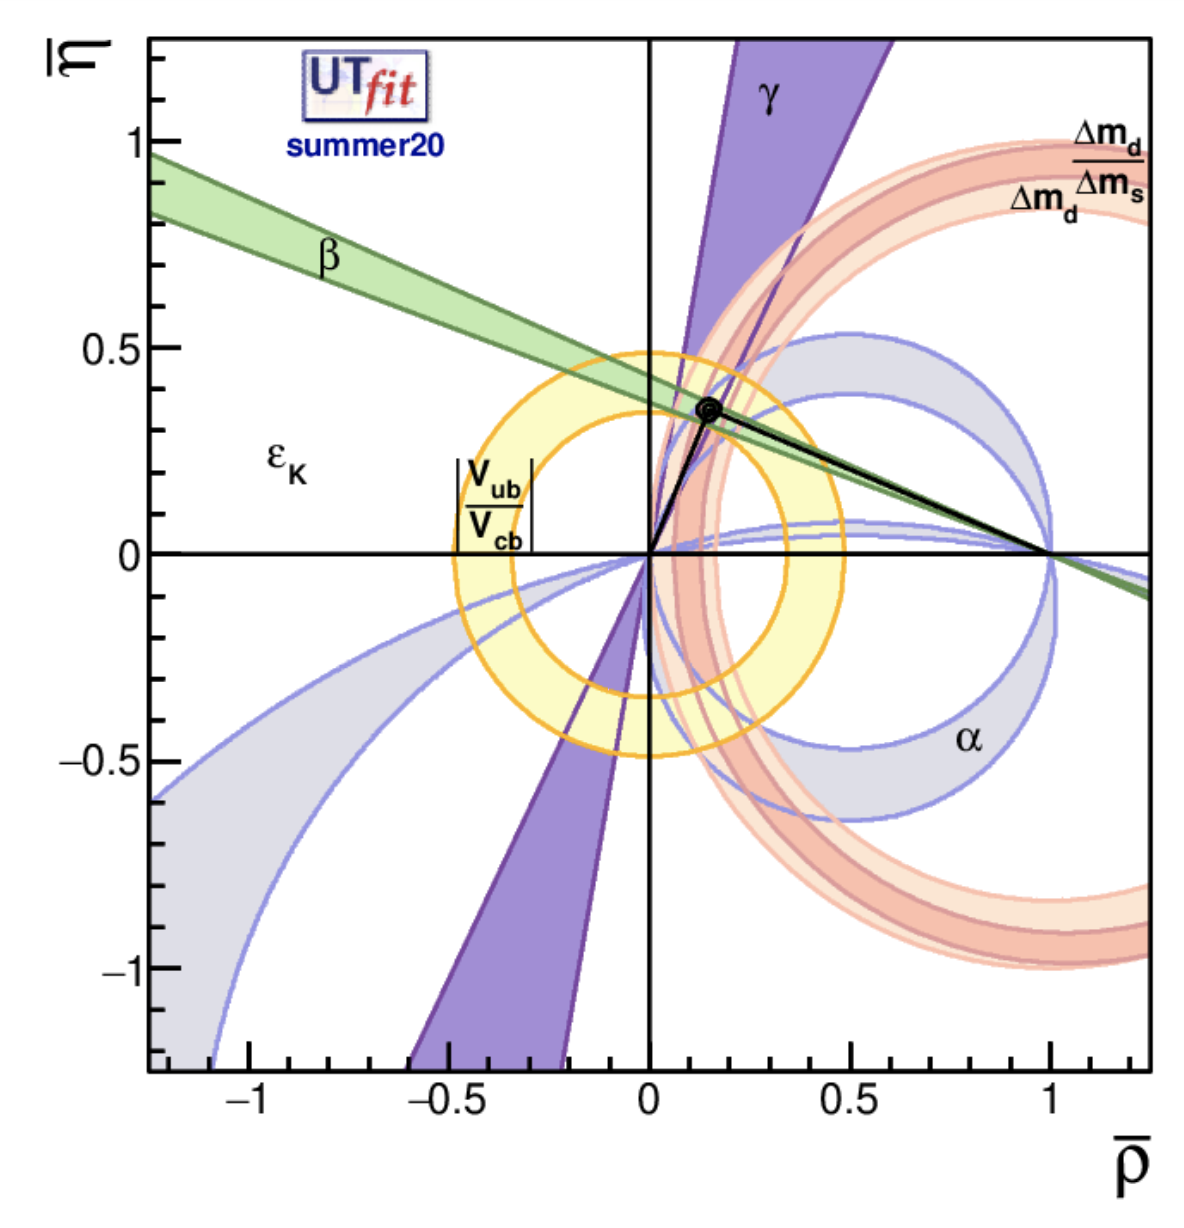
\includegraphics[scale=0.175]{figs/utfit_triangolo.png}\\
\begin{itemize}
\scriptsize
\item Analisi statistica globale
\begin{itemize}
\scriptsize
    \item $|V_{ud}|$, $|V_{us}|$, $|V_{cb}|$ e $|V_{ub}|$ dai
      decadimenti deboli di corrente carica corrispondenti
    \item $\Delta m_{d,s}$ da oscillazione $B_{d,s} - \bar{B}_{d,s}$
    \item Fasi $CP$: $\alpha$, $\beta$, $\gamma$ 
    \item Parametro violazione $CP$ $\varepsilon_K$ (oscillazioni $K - \bar{K}$)
\end{itemize}
\end{itemize}
\end{column}
\end{columns}
}

\frame{\frametitle{Settore del sapore: UT}
\begin{columns}[c]
\begin{column}{1.15\linewidth}
\centering
\scriptsize
Futuro\\
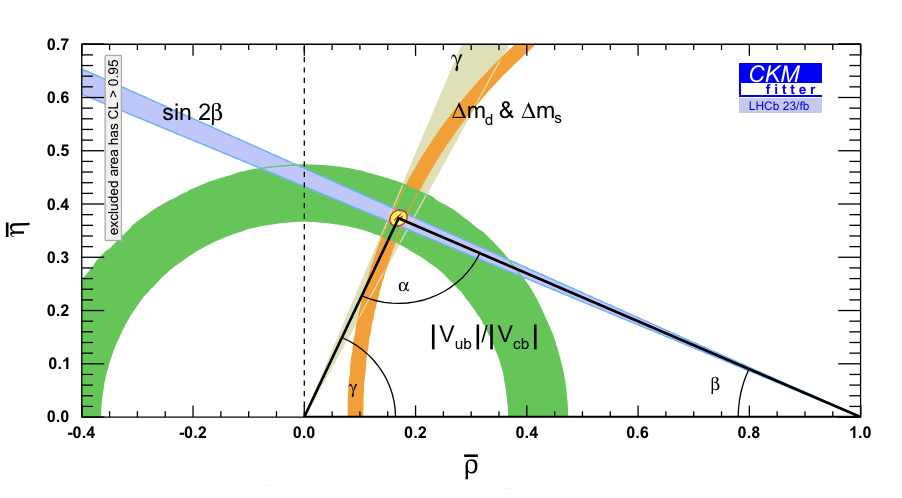
\includegraphics[scale=0.45]{figs/upgrade1.png}
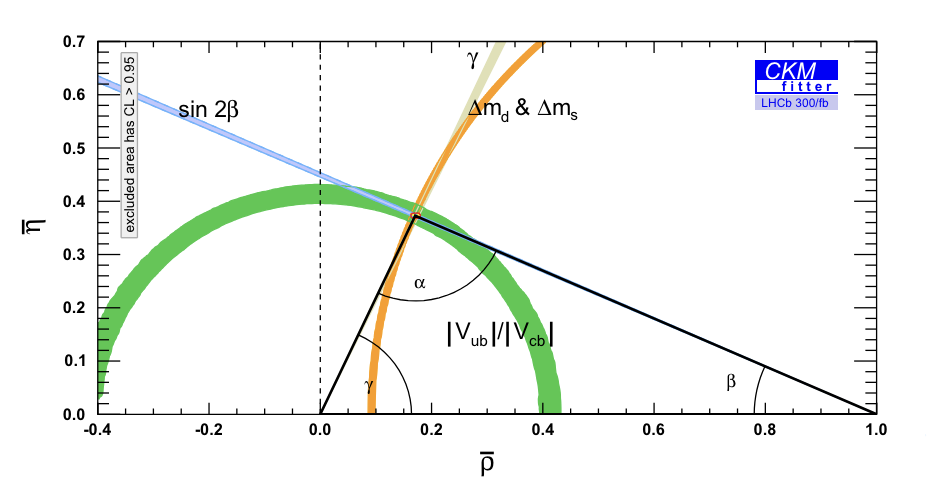
\includegraphics[scale=0.45]{figs/upgrade2.png}
\end{column}
\end{columns}
}





\frame{\frametitle{Stato attuale: fisica del sapore}
\begin{columns}[c]
\begin{column}{1.15\linewidth}
\centering
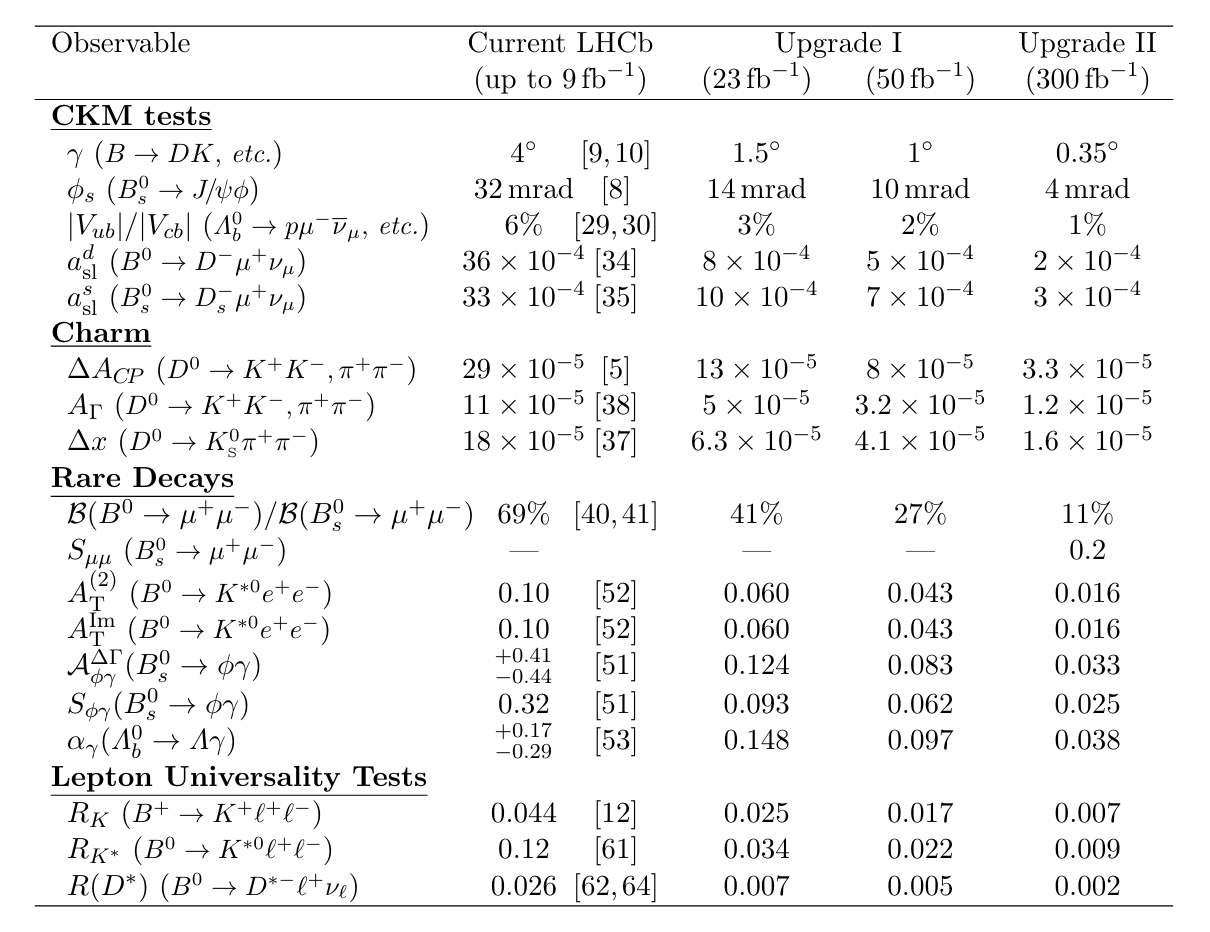
\includegraphics[scale=0.4]{figs/statomisure.png}
\end{column}
\end{columns}
}



\frame{\frametitle{Collider Futuri}
\begin{columns}[c]
\begin{column}{1.15\linewidth}
\centering
\scriptsize
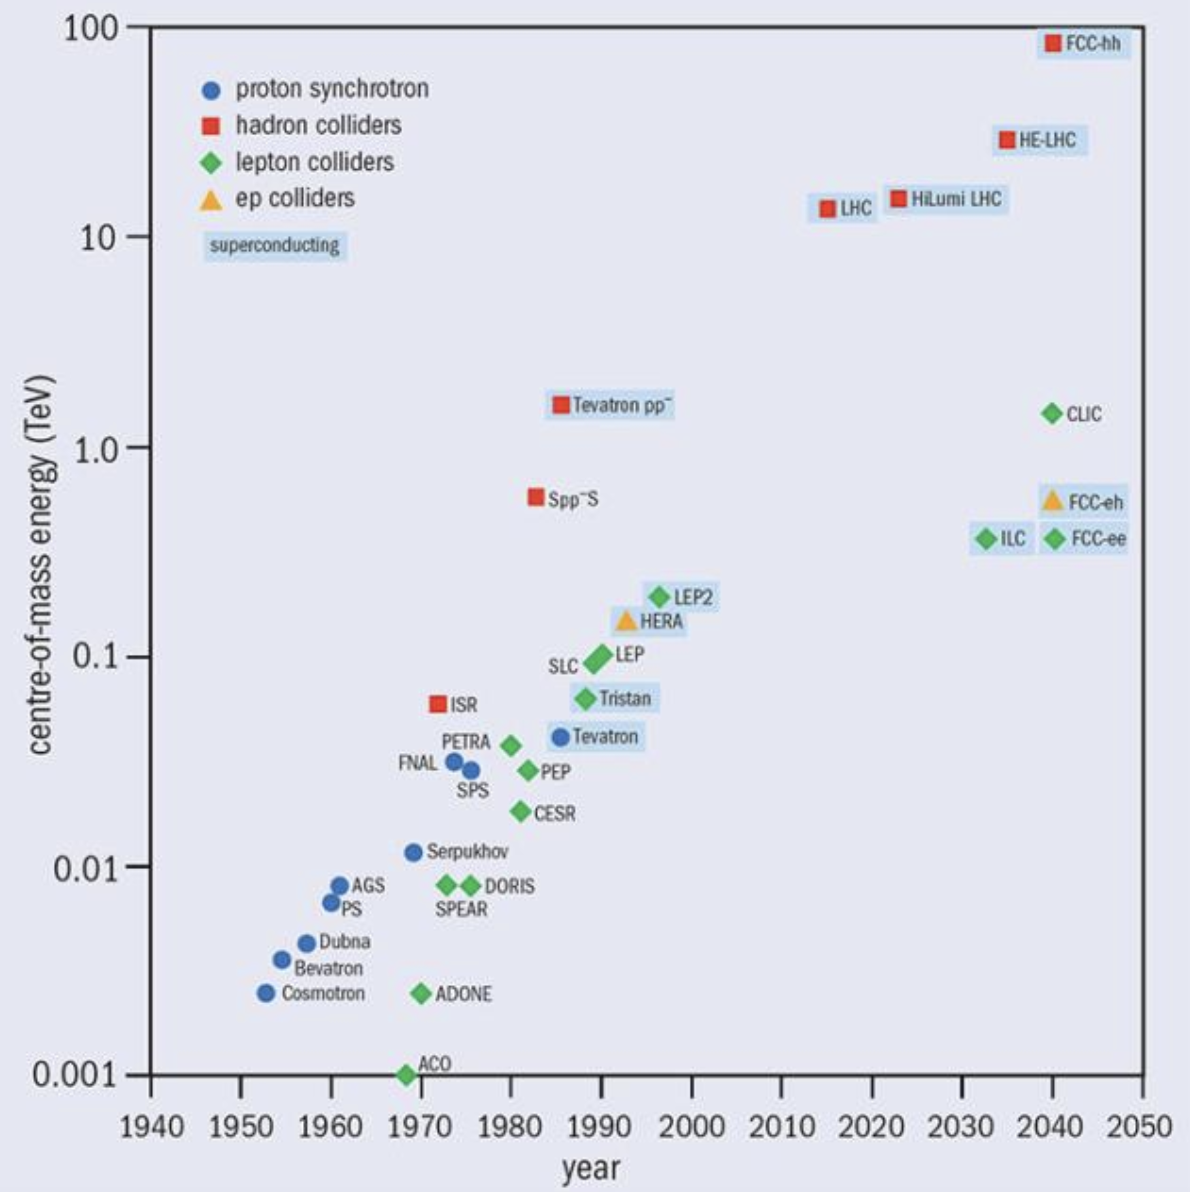
\includegraphics[scale=0.32]{figs/futurecollider1.png}\\
{\tiny Image credit L.Rossi, P.Lebrun}
\end{column}
\end{columns}
}


\frame{\frametitle{Future Circular Collider (FCC)}
\begin{columns}[c]
\begin{column}{0.5\linewidth}
\centering
\scriptsize
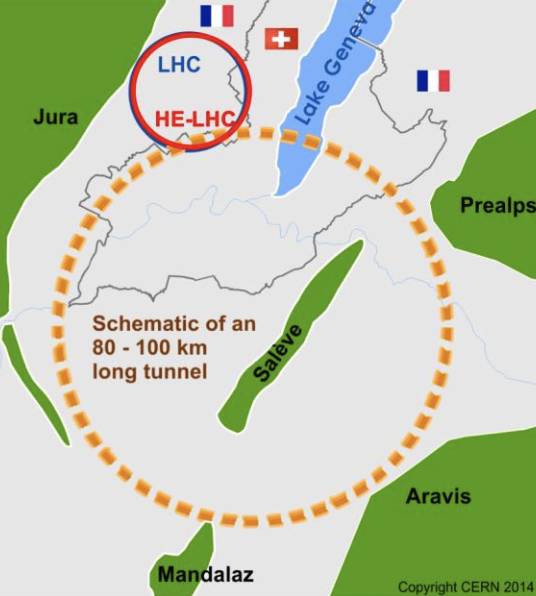
\includegraphics[scale=0.5]{figs/FCC.png}
\end{column}
\begin{column}{0.55\linewidth}
\begin{itemize}
\scriptsize
\item Collider adronico con energia nel cm di 100 TeV in un tunnel di
  100Km di circonferenza
\item Fase iniziale come collider $e^{+}e^{-}$ (FCC-ee): Higgs Factory
\item Energia: 90 ($m_{Z}$) - 365 ($2m_{top}$) GeV
\item Seconda fase collider pp (FCC-hh)
\item Energia 50 - 100 TeV
\end{itemize}
\end{column}
\end{columns}
}

\frame{\frametitle{Collider Lineare (ILC/CLIC)}
\begin{columns}[c]
\begin{column}{0.5\linewidth}
\centering
\scriptsize
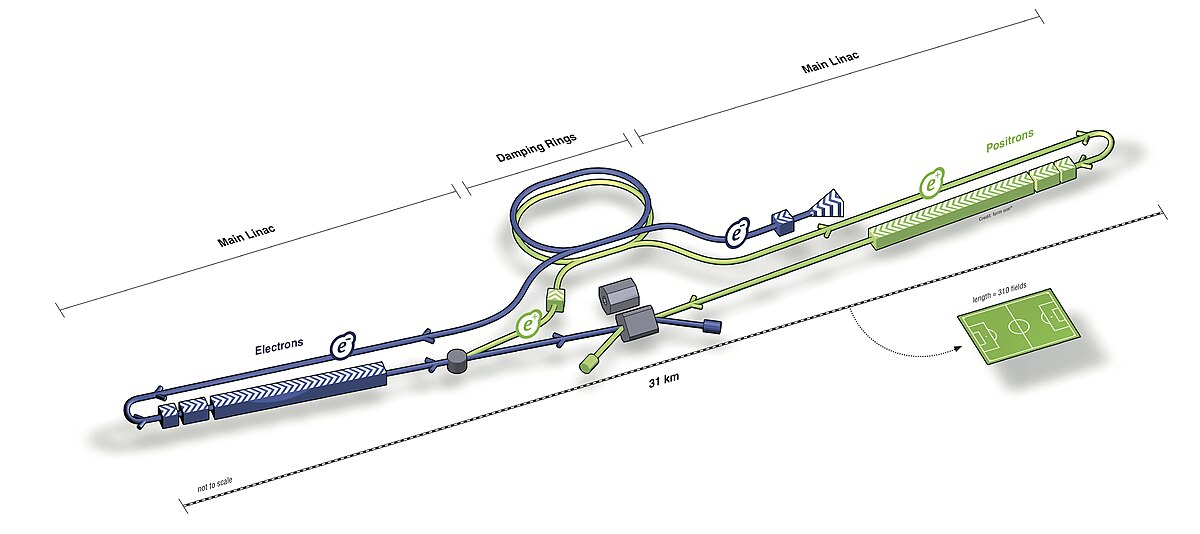
\includegraphics[scale=0.15]{figs/ILC.jpg}
\end{column}
\begin{column}{0.55\linewidth}
\centering
\scriptsize
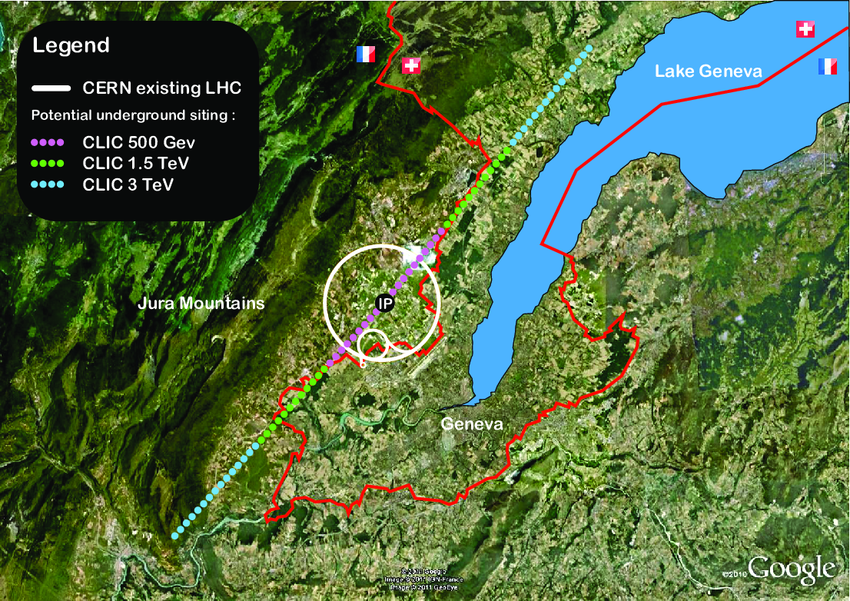
\includegraphics[scale=0.5]{figs/CLIC.png}
\end{column}
\end{columns}
\begin{itemize}
\scriptsize
\item Due acceleratori lineari di fronte l'uno all'altro
\item Collider $e^{+}e^{-}$
\item $E = 0.25$-$3$ TeV
\item $L=$11-50Km
\end{itemize}
}



\frame{\frametitle{Muon Collider}
\begin{columns}[c]
\begin{column}{1.15\linewidth}
\centering
\scriptsize
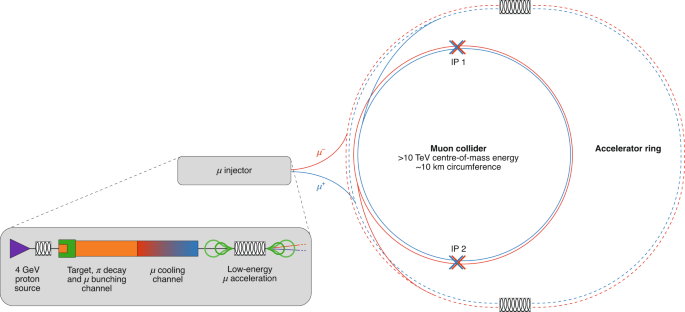
\includegraphics[scale=0.4]{figs/muoncollider.png}
\centering
\begin{itemize}
\scriptsize
\item Vantaggio: ridotta radiazione di sincrotrone
\item Sfide
\begin{itemize}
\scriptsize
\item Produzione fascio ad alta luminosit\`a
\item Particelle instabili 
\item Energia $E = 3$-$10$ TeV
\end{itemize}
\end{itemize}
\end{column}
\end{columns}
}


%\frame{\frametitle{Violazione di CP oltre il MS}
%\begin{columns}[c]
%\begin{column}{1.15\linewidth}
%\begin{itemize}
%\scriptsize
%\item In principio la struttura delle interazioni forti permetterebbe
%  violazione di CP
%\item Il valore del parametro che tiene conto della violazione di CP nelle
%  interazioni forti non \`e predetto dalla teoria ma \`e un parametro
%  libero da misurare
%\item Tuttavia, la presenza di interazioni che violano CP nella QCD
% indurrebbe un momento di dipolo elettrico del neutrone
%\item Limiti sul non osservato momento di dipolo elettrico del
%  neutrone implicano che la violazione di CP sia estremamente piccola
%  e quindi il parametro che quantifica la violazione di CP forte sia
%  piccolo
%\item Sorge un problema di naturalezza: perch\`e il parametro \`e
%  cos\`i piccolo? 
%\item Una delle possibili soluzioni \`e dato dalla teoria di
%  Peccei-Quinn che prevede l'esistenza di una ipotetica particella: assione
%\end{itemize}
%\end{column}
%\end{columns}
%}

%\frame{\frametitle{Misure di precisione: flavour physics}


%}






\frame{\frametitle{Dark Matter}
\begin{columns}[c]
\begin{column}{1.15\linewidth}
\begin{itemize}
\item Fisica
  oltre il Modello Standard: esistenza della Dark Matter nell'Universo
\item Una consistente frazione di massa dell'Universo non \`e
  dovuta alla materia standard 
\item L'evidenza diretta dell'esistenza della materia oscura \`e data
  dalla distribuzione delle velocit\`a delle stelle che orbitano
  intorno al centro di una galassia
\end{itemize}
\end{column}
\end{columns} 

}






\frame{\frametitle{Esistenza di Dark Matter - Rotazione galassie}
\begin{columns}[c]
\begin{column}{0.55\linewidth}
\centering
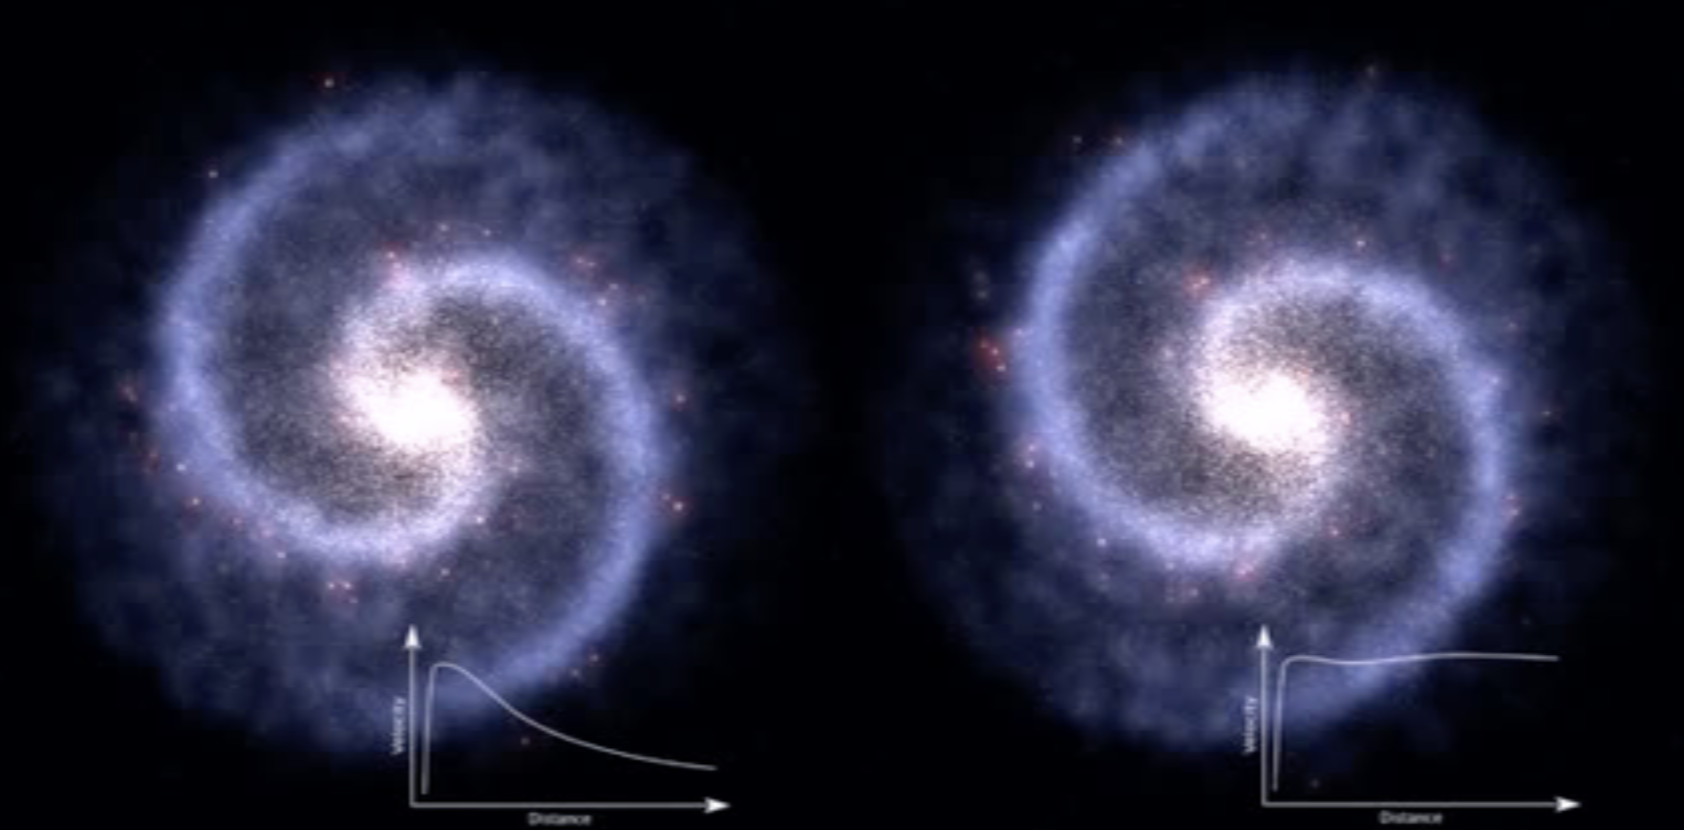
\includegraphics[scale=0.175]{figs/galassie.png}
\end{column}
\begin{column}{0.55\linewidth}
\centering
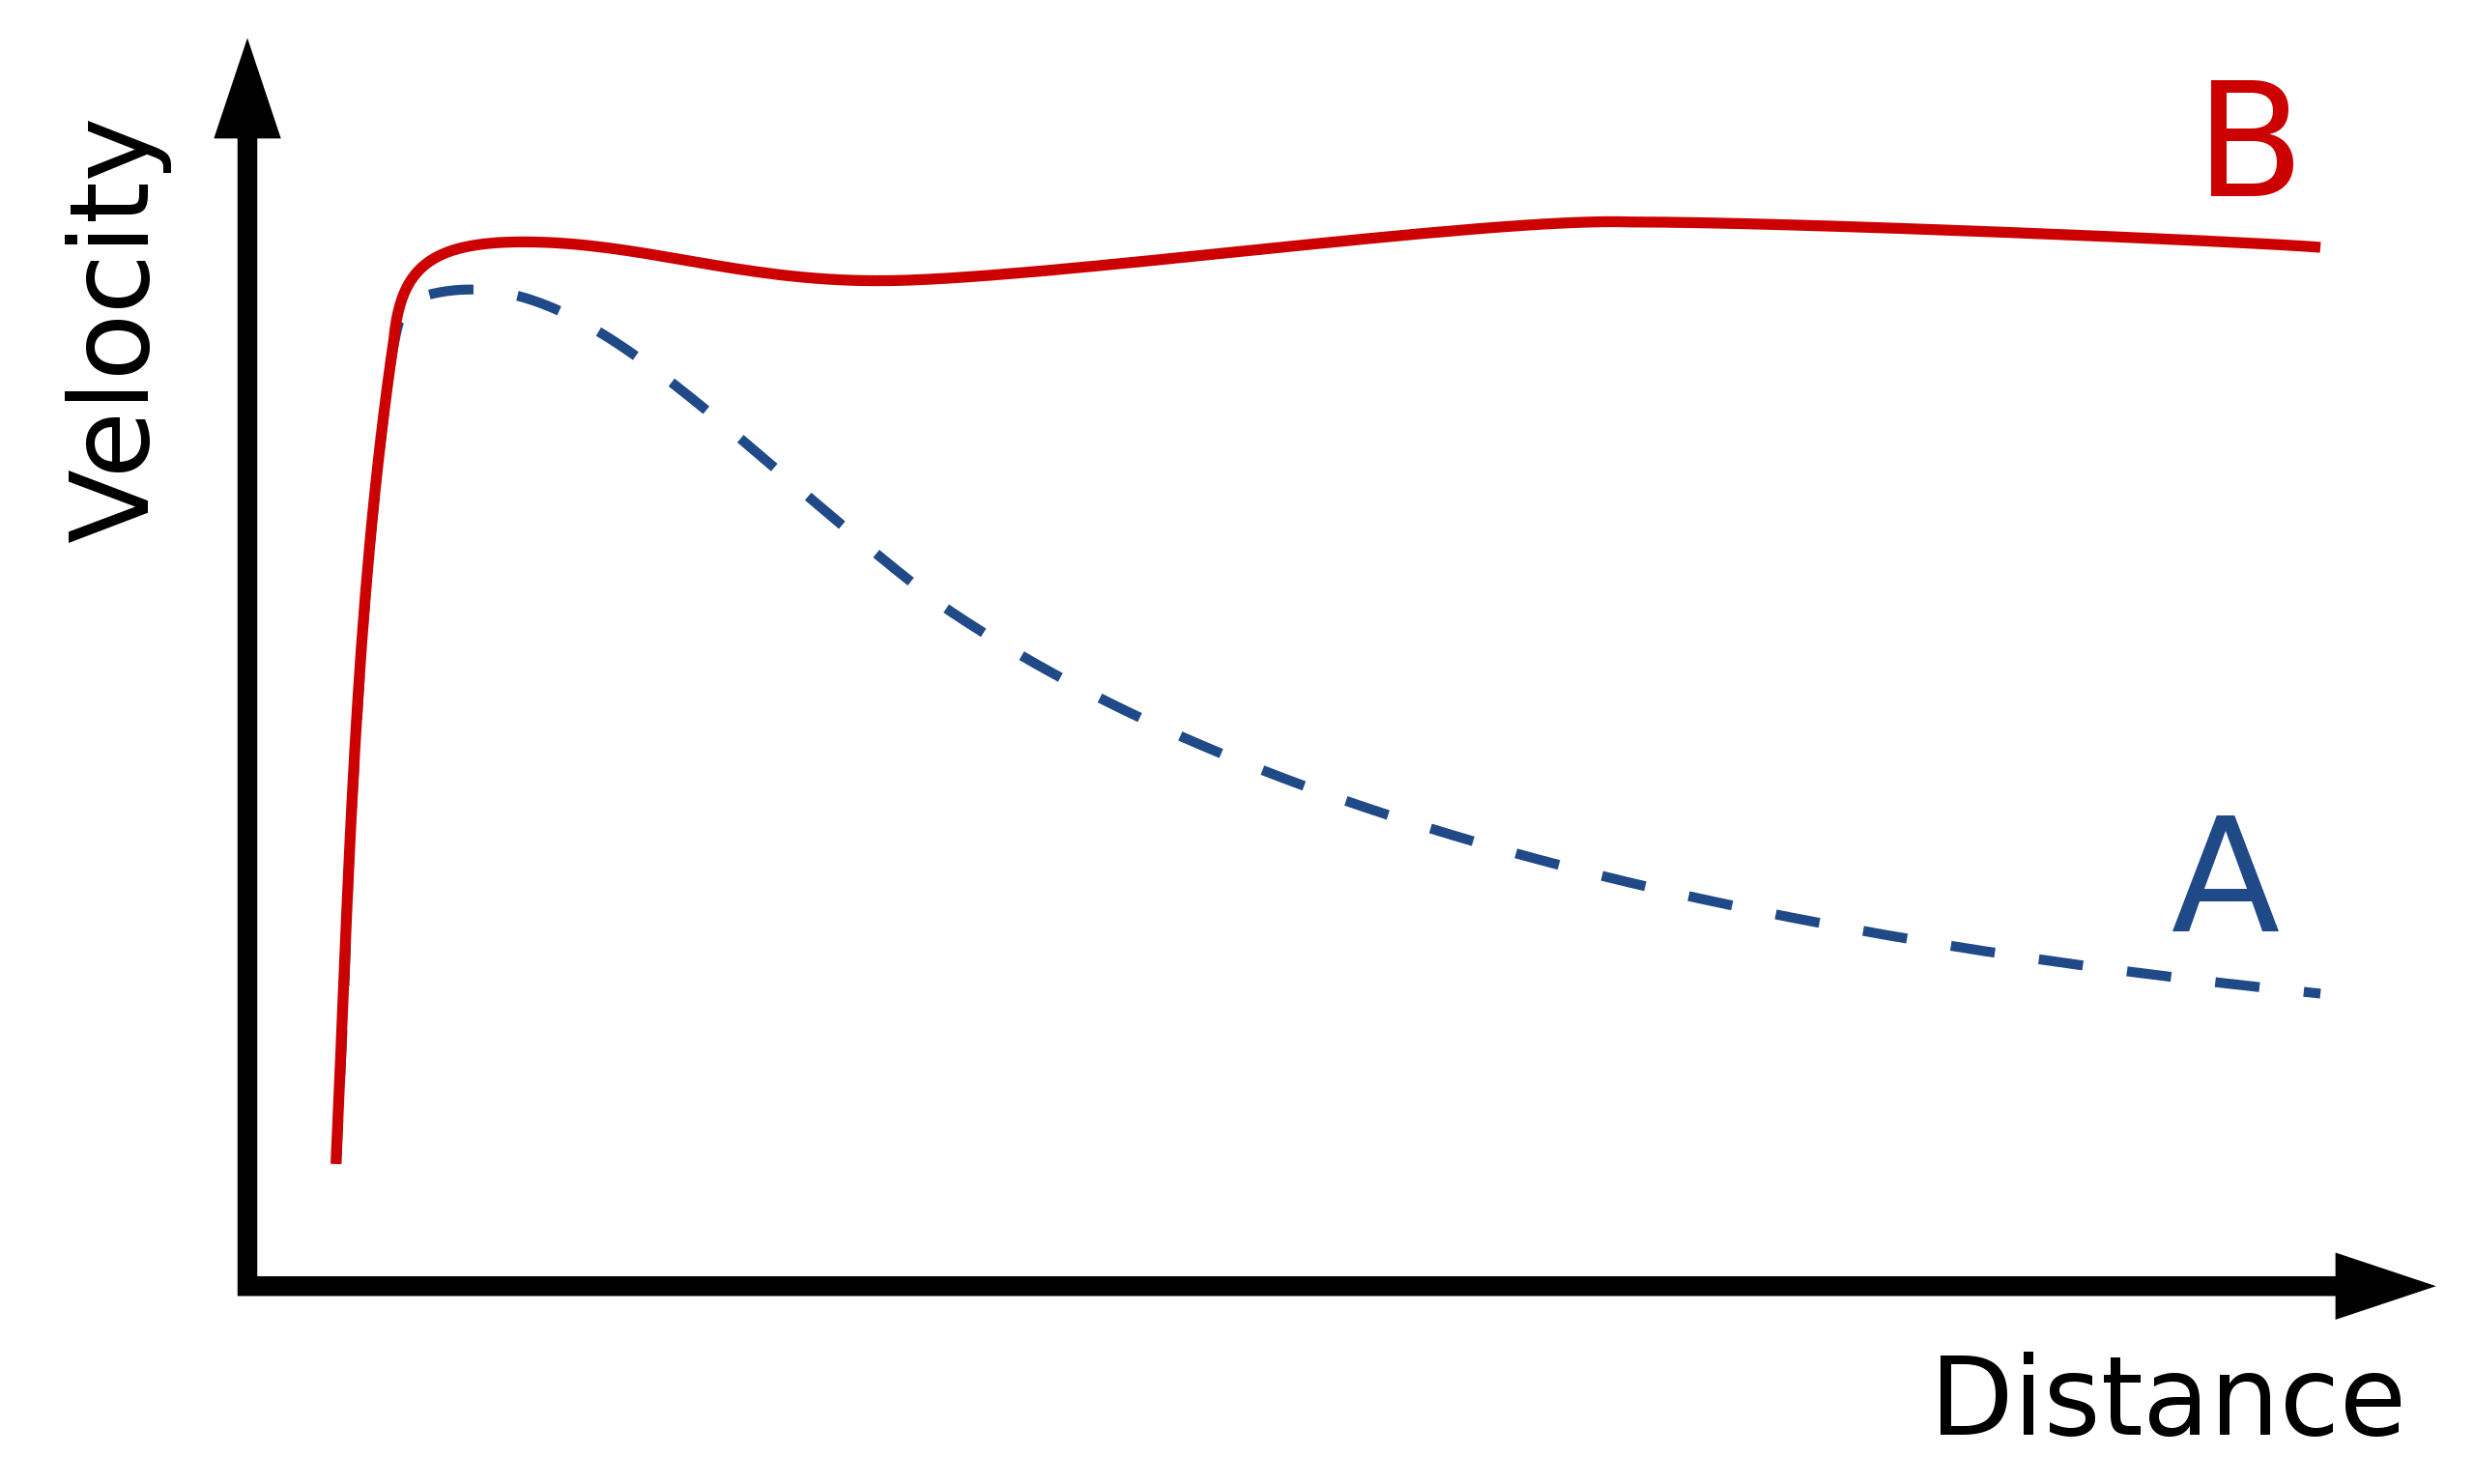
\includegraphics[scale=0.06]{figs/rotationgalaxy.png}
\end{column}
\end{columns}
\begin{columns}[c]
\begin{column}{1.15\linewidth}
\begin{itemize}
\scriptsize
\item Se guardiamo alla distribuzione di materia luminosa in una
  galassia, notiamo che \`e concentrata nel centro della galassia
\item La velocit\`a tangente di una stella di massa $m$ \`e
  data da: 
$ \frac{mv^{2}}{r} \approx \frac{Gm}{r^{2}}M(r)$
\item Se assumiamo che la maggior parte della massa sia concentrata
  nel centro la velocit\`a delle stelle: $v \propto \frac{1}{\sqrt{r}}$ [A]
\item Questo non \`e consistente con le osservazioni che invece
  mostrano un andamento piatto che implica $M(r) \propto r$ [B]
\item Prova che la massa di una galassia ha una componente non
  luminosa significativa:  la dark matter non emette n\`e assorbe
  radiazione elettromagnetica, pu\`o essere determinata solo
  attraverso i suoi effetti gravitazionali.
\end{itemize}
\end{column}
\end{columns}
}

\frame{\frametitle{Esistenza di Dark Matter - CMB}
\begin{columns}[c]
\begin{column}{1.15\linewidth}
\begin{itemize}
\scriptsize
\item Altre evidenze di materia oscura da misure cosmologiche  legate
  alla struttura su larga scala dell'Universo e in particolare le
  misure precise delle anisotropie nella radiazione cosmica di fondo
  (Cosmic Microwave Background, CMB) da parte dei satelliti COBE,
  WMAP, Planck
%\item Nelle fasi iniziali dell'Universo, a temperature $T >
%  3000\unitm{K} \sim 0.3 \unitm{eV}$, c'erano un sufficiente numero di fotoni con
%  un'energia sufficiente a ionizzare l'idrogeno
%\item Appena un protone e un elettrone si combinano a formare un atomo
%  neutro di idrogeno, un fotone ionizza l'atomo
\item La radiazione cosmica di fondo ci fornisce un'immagine
  dell'Universo quando la sua temperatura scende ($T < 3000K$) da
  permettere la formazione di atomi di idrogeno combinando protoni e elettroni%, i fotoni non hanno
  %pi\`u energia sufficiente per distruggere gli atomi di idrogeno e
 \item l'Universo diventa trasparente ai fotoni che si propagano fino
   ad oggi
\end{itemize}
\centering
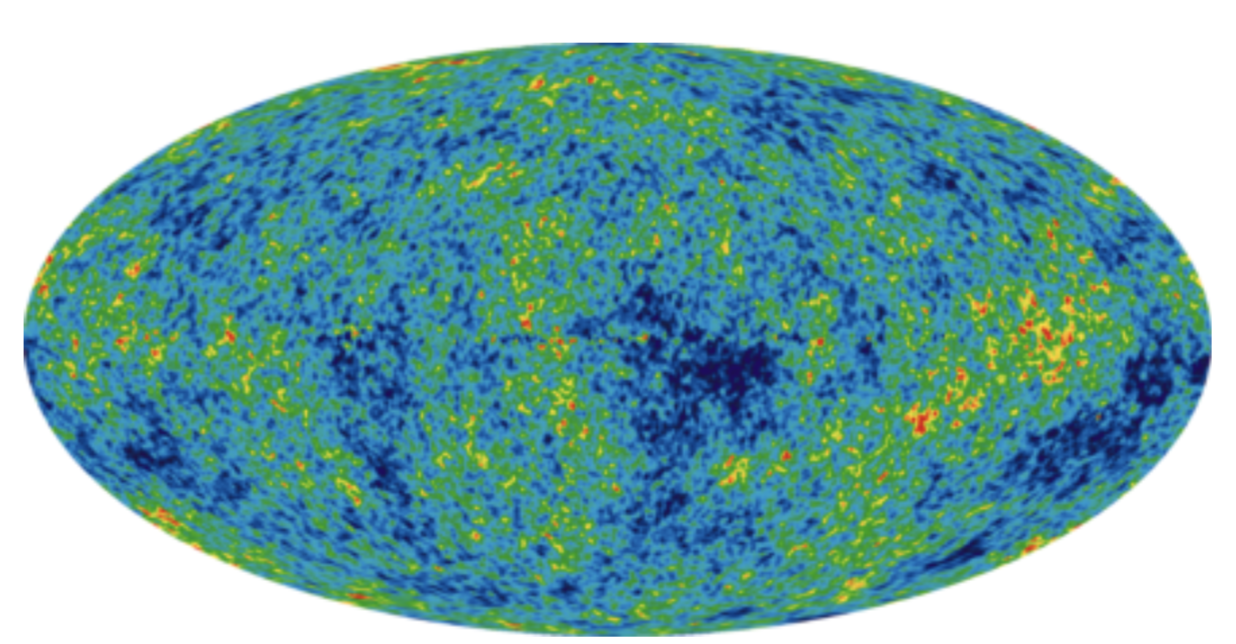
\includegraphics[scale=0.25]{figs/cmb.png}
\end{column}
\end{columns}
}

\frame{\frametitle{Esistenza di Dark Matter - CMB}
\begin{columns}[c]
\begin{column}{1.15\linewidth}
\begin{itemize}
\scriptsize
\item La CMB ha uno spettro di corpo nero ad una temperatura di 2.725K
\item Contiene anisotropie ad un livello di $10^{-5}$: perturbazioni
  nella densit\`a nell'Universo primordiale
\item Dallo studio dello spettro della CMB \`e possibile estrarre i
  parametri cosmologici
\end{itemize}
\centering
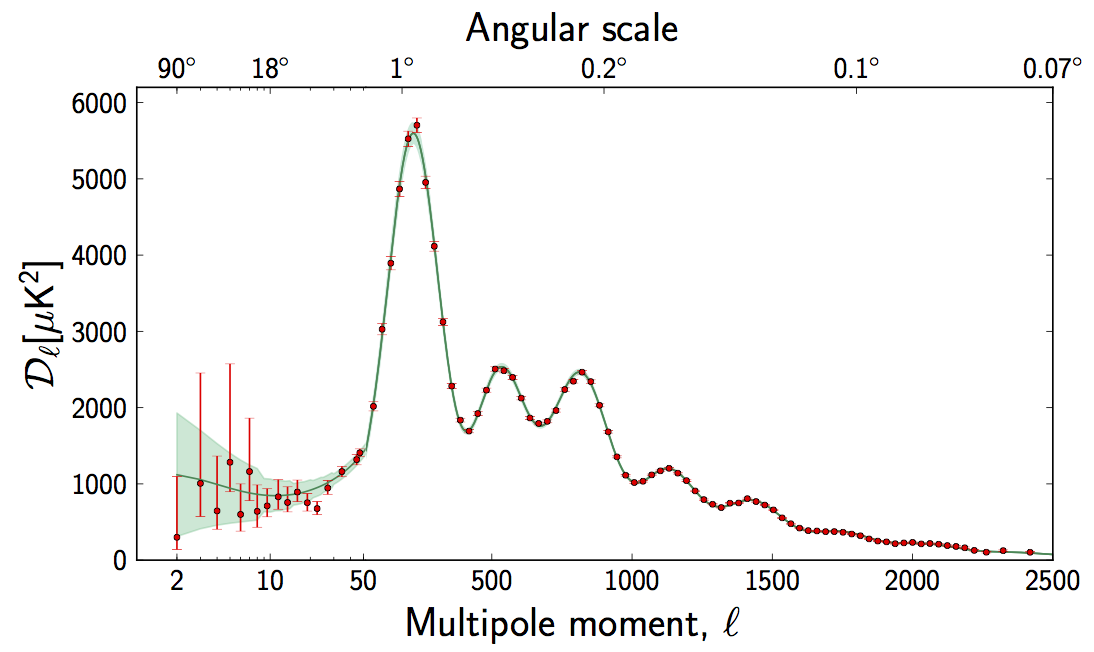
\includegraphics[scale=0.3]{figs/cmbspectrum.png}
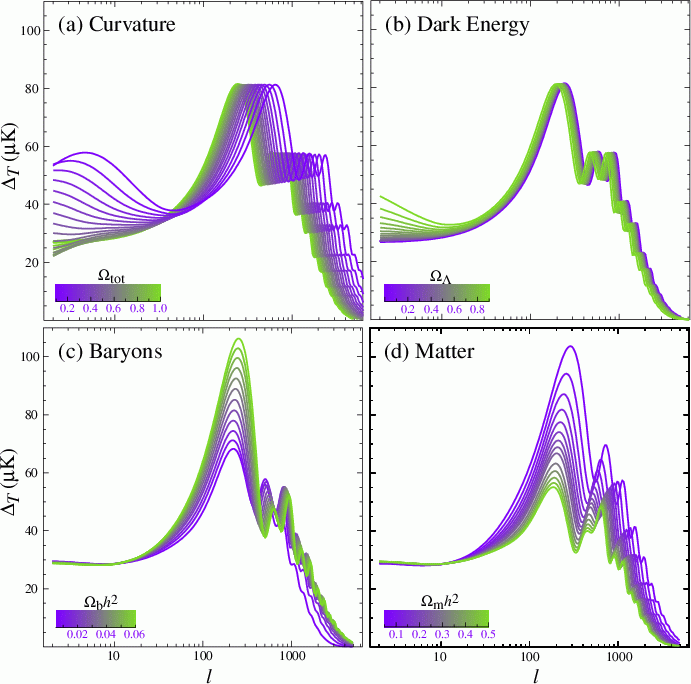
\includegraphics[scale=0.2]{figs/0110414_plate4.png}
\end{column}
\end{columns}
}

\frame{\frametitle{Esistenza di Dark Matter - CMB}
\begin{columns}[c]
\begin{column}{1.15\linewidth}
\centering
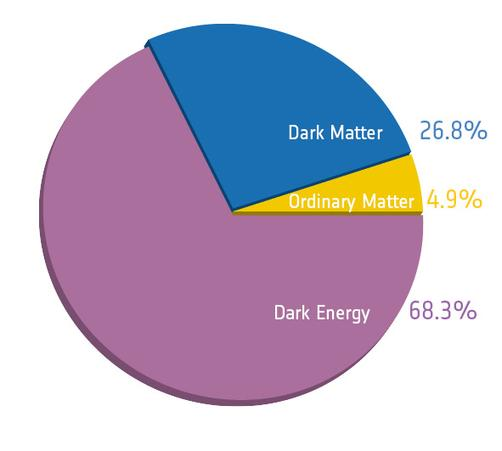
\includegraphics[scale=0.175]{figs/planck.jpg}
\begin{itemize}
\item Solo il 5\% della densit\`a di materia-energia dell'Universo \`e
  nella forma di materia barionica standard
\item $\sim 23\%$: materia oscura (DM)
\item $\sim 72\%$: energia oscura (tende ad accelerare l'espansione dell'Universo)
\item La maggior parte della DM \`e dovuta a ``cold'' (non relativistica) DM
\end{itemize}
\end{column}
\end{columns}
}




\frame{\frametitle{Candidati di Dark Matter}
\begin{columns}[T]
\begin{column}{0.6\linewidth}
\begin{itemize}
\scriptsize
\item Particelle stabili, elettricamente neutre, non-relativistiche con masse da qualche
  MeV alla scala elettrodebole, debolmente interagenti
\item Il MS non fornisce un candidato ottimale di DM: i neutrini hanno una massa molto piccola per cui sono
  relativistici (in un Universo dominato da neutrini non si
  osserverebbero le strutture su larga scala delle galassie)
\item Sono stati proposti diversi candidati di Dark Matter (largo
  range di possibili masse e accoppiamenti)
\item Le Weakly Interacting Massive Particles (WIMPs) sono una classe
  promettente di candidati di dark matter (ma non l'unica, altre sono
  dark-sector models, ...): masse dal GeV al TeV e
  accoppiamenti simili a quelli della forza debole
\item Queste particelle sono previste in molte estensioni del Modello
  Standard
\item Per esempio in modelli supersimmetrici il neutralino, la particella pi\`u leggera
  stabile \`e un candidato di DM
%\item Le misure cosmologiche mettono un limite sulle masse del
%  neutrino: $\sum_{i=1}^{3} m_{\nu_{i}} \lesssim 1 $
\end{itemize}
\end{column}
\begin{column}{0.55\linewidth}
\centering
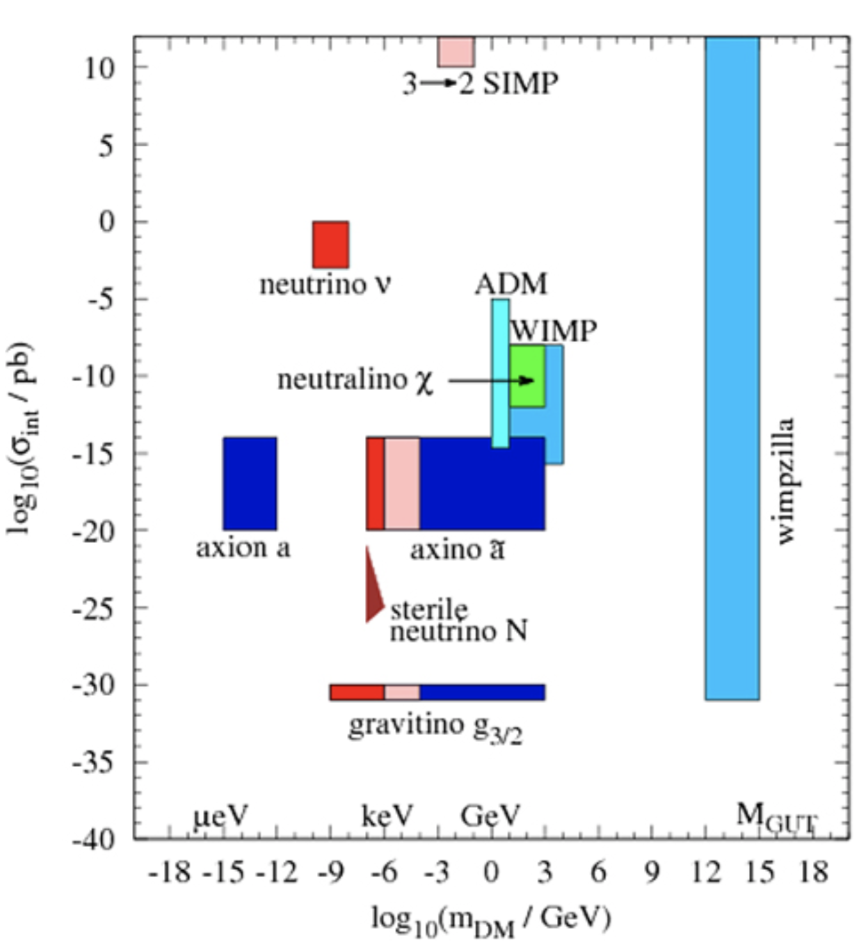
\includegraphics[scale=0.4]{figs/dmcandidates.png}
\end{column}
\end{columns}
}


\frame{\frametitle{Come si effettua la ricerca di DM?}
\begin{columns}[c]
\begin{column}{1.0\linewidth}
\centering
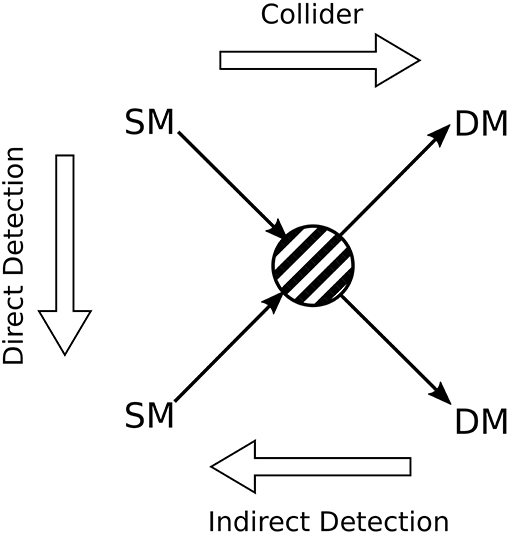
\includegraphics[scale=0.25]{figs/DMsearch1.jpg}\\
\scriptsize
La ricerca di Dark Matter avviene con diverse tecniche
  sperimentali a seconda della sezione d'urto e della massa della particella
\begin{itemize}
\scriptsize
\item Produzione agli acceleratori di particelle (necessaria energia
  sufficiente a produrre la particella di DM)
\item Ricerca indiretta da prodotti di annichilazione (rivelazione dei
  prodotti di decadimento come neutrini ad alta energia, fotoni,
  leptoni carichi da processi di annichilazione di dark matter)
\item Ricerca diretta attraverso lo scattering su nuclei
\end{itemize}
\end{column}
\end{columns}
}

\frame{\frametitle{Dark Matter @ Collider - Dark Sector}
\begin{columns}[c]
\begin{column}{1.15\linewidth}
\begin{itemize}
\item Una possibilit\`a \`e che la DM non interagisca direttamente con
  la materia ordinaria facendo parte di un settore oscuro di
  particelle e forze che esistono completamente separate ma parallelo
  a quelle che conosciamo
\end{itemize}
\begin{center}
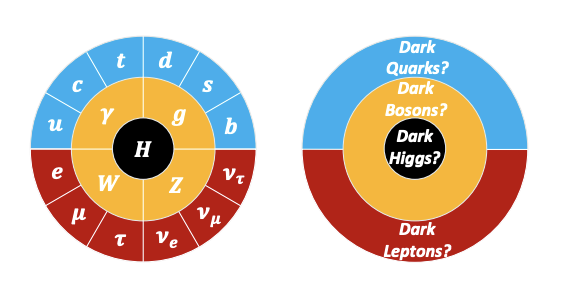
\includegraphics[scale=0.5]{figs/darksector.png}
\end{center}
\begin{itemize}
\item Possibile accedere al settore dark attraverso un portale: un
  processo raro che stabilisce una connessione tra le particelle
  ordinarie e quelle dark
\begin{itemize}
\item Portale dei fotoni
\item Portale dei neutrini
\item Portale di Higgs
\end{itemize}
\end{itemize}
\end{column}
\end{columns}
}

\frame{\frametitle{Fotoni Dark}
\begin{columns}[c]
\begin{column}{1.15\linewidth}
\begin{itemize}
\scriptsize
\item Fotone dark massivo $A^{'}$ come portale: opzione pi\`u accreditata per modelli di DM
  leggera
\item Si comporta come $\gamma^{*}$ ma con accoppiamenti soppressi
  per un fattore $\epsilon$
\item Ricerca di decadimenti $A^{'} \to \mu^{+}\mu^{-}$
  all'esperimento LHCb a LHC
\end{itemize}
\begin{center}
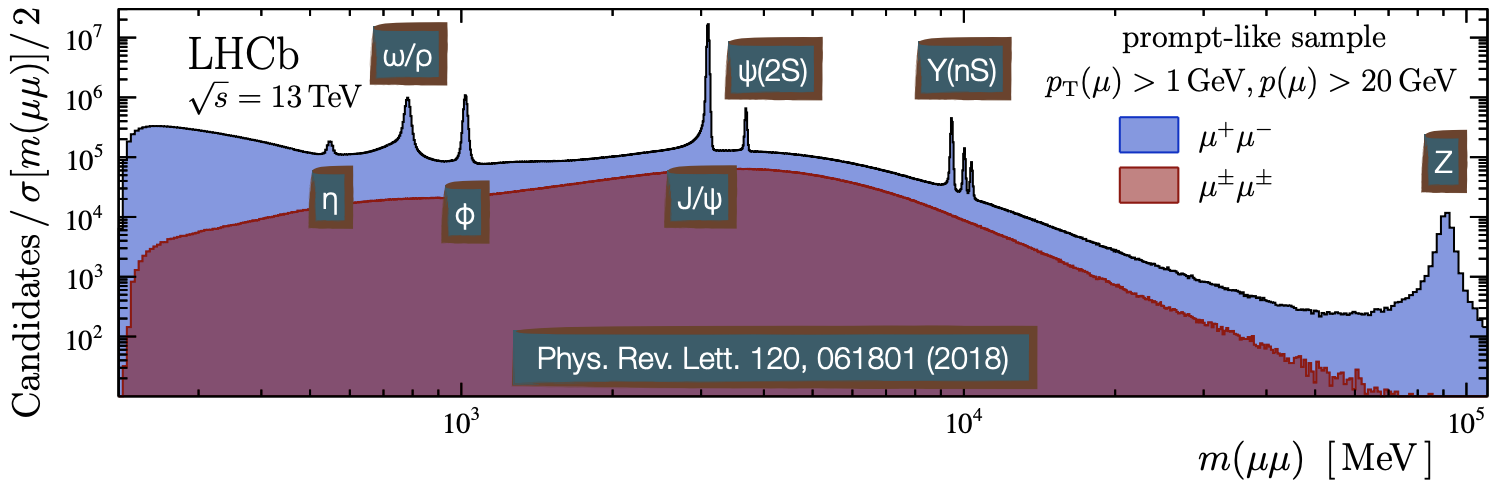
\includegraphics[scale=0.3]{figs/darkphotonmass.png}\\
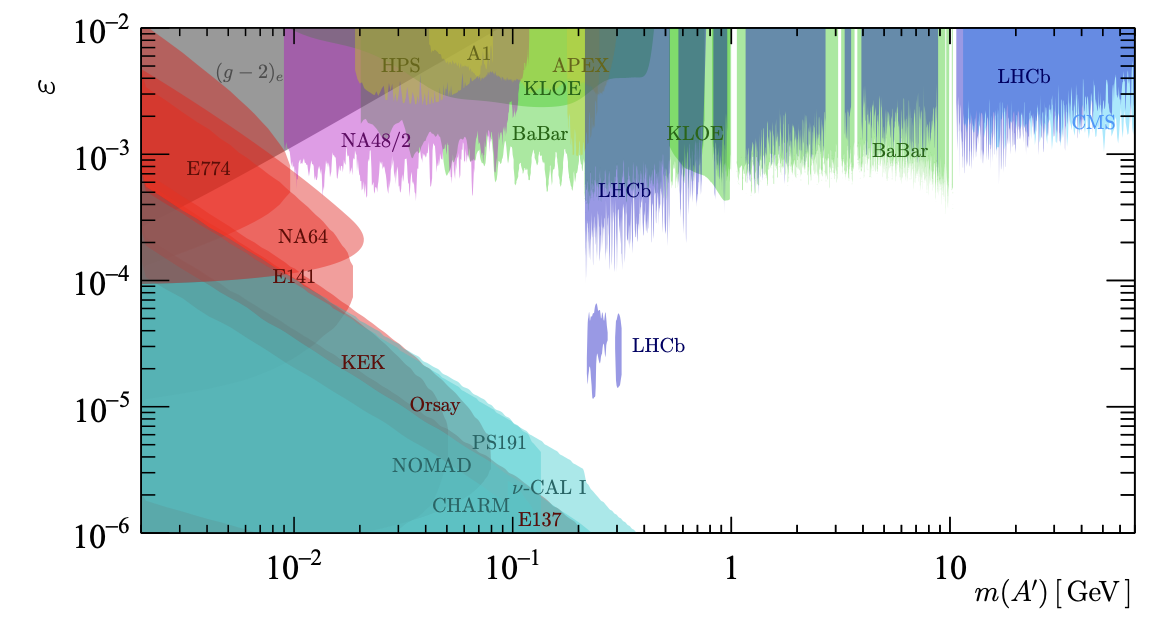
\includegraphics[scale=0.3]{figs/exclusionplot.png}
\end{center}
\end{column}
\end{columns}
}



\frame{\frametitle{Ricerca diretta di DM (I)}
\begin{columns}[c]
\begin{column}{0.55\linewidth}
\begin{itemize}
\scriptsize
\item La rivelazione diretta di WIMP \`e molto difficile
  sperimentalmente
\item L'interazione con la materia standard avviene per scattering
  elastico su nuclei: $\chi + N \to \chi +N$
\end{itemize}
\end{column}
\begin{column}{0.55\linewidth}
\centering
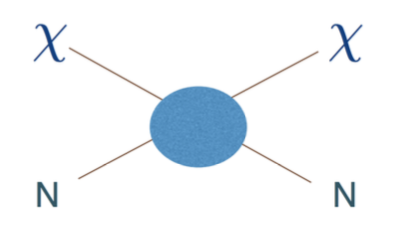
\includegraphics[scale=0.35]{figs/scattering.png}
\end{column}
\end{columns}
\begin{columns}[c]
\begin{column}{1.0\linewidth}
\begin{itemize}
\scriptsize
\item L'idea \`e di rivelare il rinculo del nucleo dopo il processo
  di scattering con DM
\item Massima energia cinetica trasferita:\\ 
$T_{max} \sim \frac{4Am_{\chi}m_{P}}{(m_{\chi}+Am_{P})^2}T_{\chi}$ con $T_{\chi}
\sim 3 \times 10^{-7} m_{\chi}$\\
\`e dell'ordine di $1$-$100\unitm{keV}$ per $m_{\chi} \sim
10$-$100\unitm{GeV}$ $\to$ {\bf Necessit\`a di utilizzare rivelatori
  molto sensibili con elevate risoluzioni}
\item Tenendo conto della densit\`a di WIMPs
  atteso e delle piccole sezioni d'urto: i rate di eventi attesi sono
  molto bassi (qualche evento per anno in un rivelatore di
  $1\unitm{tonn}$) $\to$ {\bf Necessit\`a di rivelatori
    molto grandi e necessario avere un livello di fondo molto basso}
\begin{itemize}
\scriptsize
\item Raggi cosmici (laboratori sotterranei)
\item Radioattivit\`a naturale e nei materiali del rivelatore
  (schermatura rivelatore, utilizzo materiali molto puri, tecniche di discriminazione)
\item Scattering di neutrino su nucleo
\end{itemize} 
\end{itemize}
\end{column}
\end{columns}
}


\frame{%\frametitle{Ricerca diretta di DM}
%\begin{columns}[c]
%\begin{column}{1.15\linewidth}
%\centering
%\scriptsize%
%Diversi possibili modi di rivelare il rinculo del nucleo
%\end{column}
%\end{columns}
\begin{columns}[T]
\begin{column}{0.5\linewidth}
\begin{itemize}
\footnotesize
\item Scintillatori a gas nobile
  liquido (Xenon liquido)
\begin{itemize}
\scriptsize
\item WIMPs interagendo con gas nobili liquidi producono luce di scintillazione
  (S1)
\item In rivelatori a doppia fase: elettroni soggetti ad un campo
  elettrico verso
  l'interfaccia liquido-gas: segnale ionizzazione del gas (S2)
\item Ricostruzione 3D: distribuzione x-y dalla posizione sui PMT e
  ``z'' dal tempo di drift
\end{itemize}
\end{itemize}
\centering
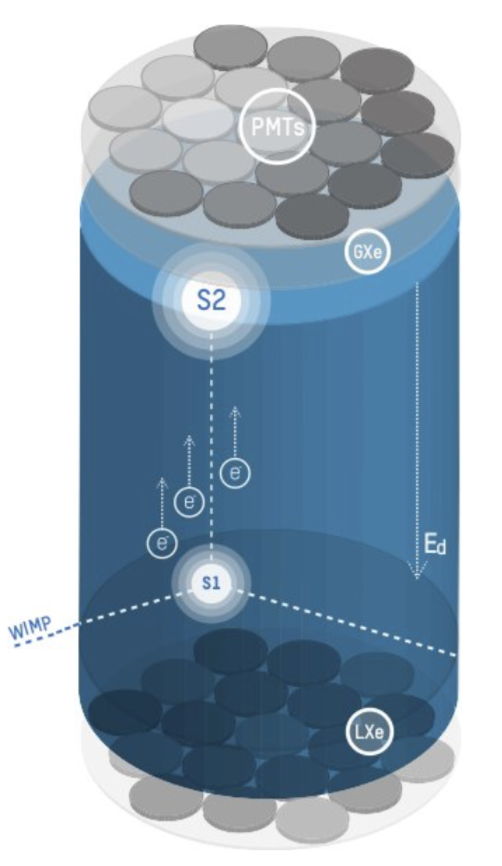
\includegraphics[scale=0.225]{figs/DMexperiment1.png}
\end{column}
\begin{column}{0.65\linewidth}
\begin{itemize}
\footnotesize
\item Rivelatori criogenici a $T \sim mK$ (bolometri)
\begin{itemize}
\scriptsize
\item Costituiti da un cristallo assorbitore
  e da un sensore che misura l'energia rilasciata nell'interazione
\item Il sensore rileva la piccola quantit\`a di energia rilasciata
  misurando la variazione di temperatura dovuta all'energia convertita
  in fononi (energia termica).
\item Si tratta di un aumento di temperatura di qualche
  decina/centinaia di $\mu K$ per MeV
\item Si utilizzano sensori a transizione di fase
  superconduttiva
\item Ottimali per ricerche di DM nel range $< GeV$
\end{itemize}
\end{itemize}
\centering
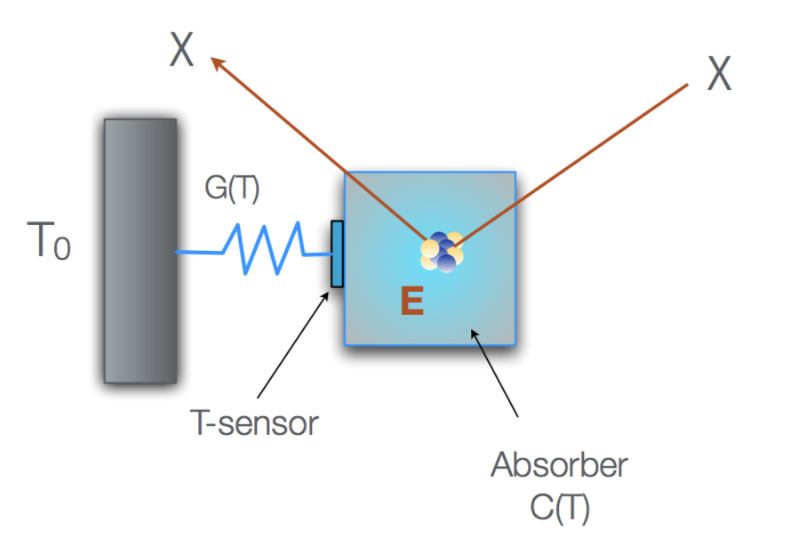
\includegraphics[scale=0.25]{figs/DMexperiment2.png}\\

\end{column}
\end{columns}
}


\frame{\frametitle{Rivelatori a gas nobili liquidi}
\begin{columns}[c]
\begin{column}{1.15\linewidth}
\centering
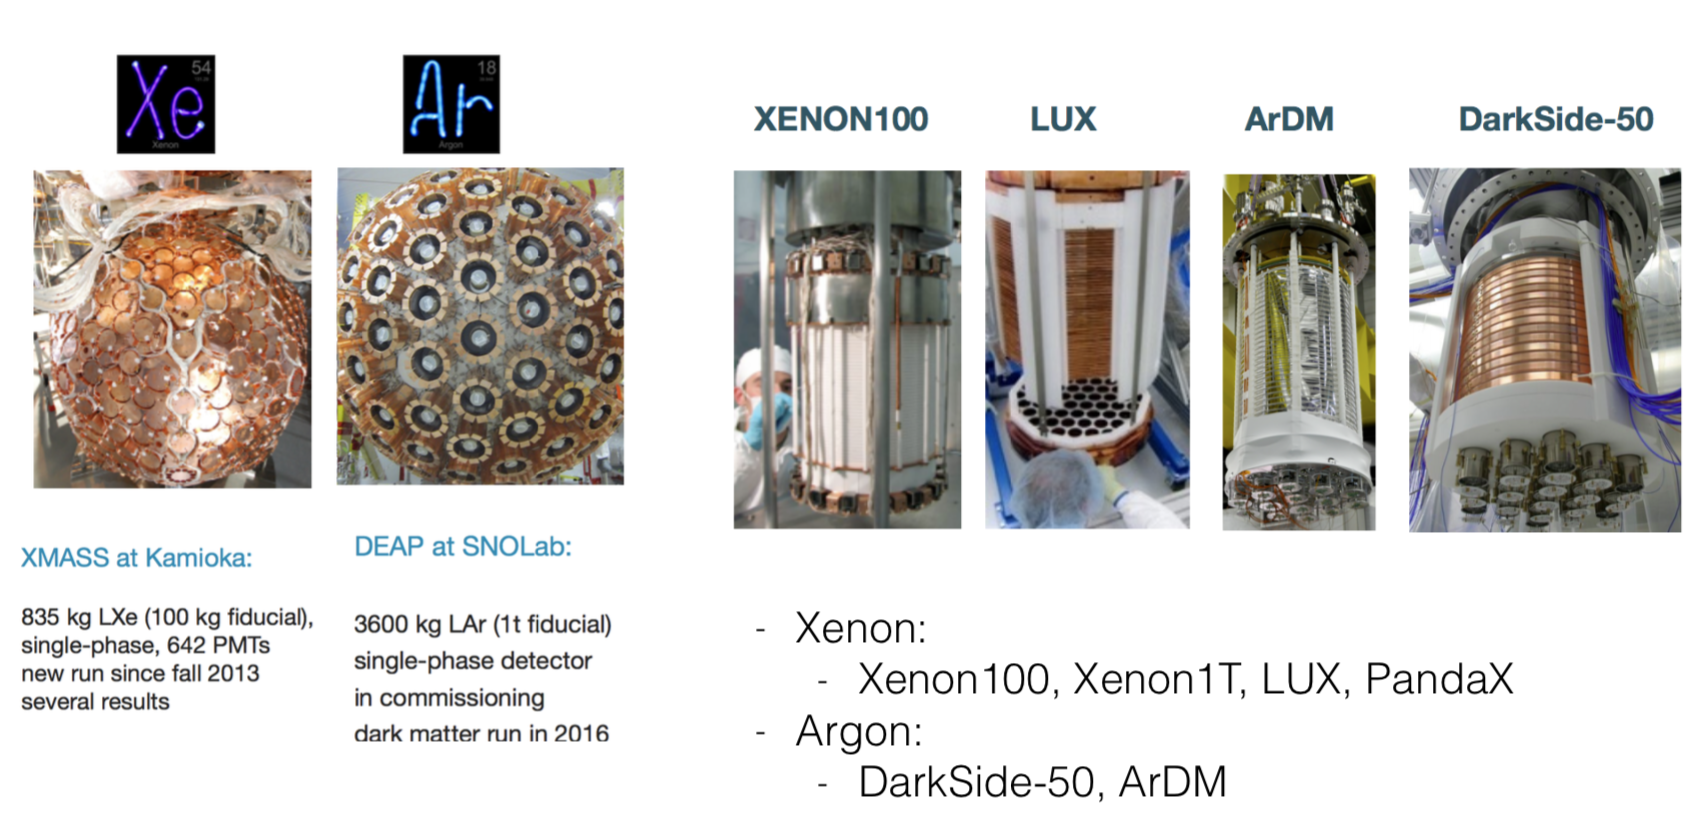
\includegraphics[scale=0.3]{figs/nobelgasesdetector.png}\\
Nuova generazione\\
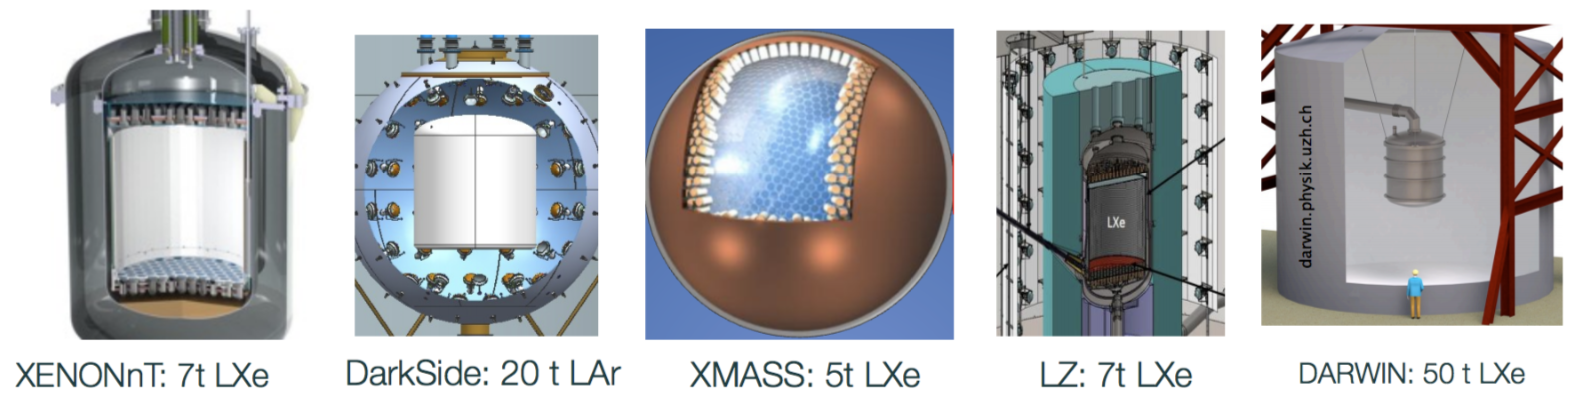
\includegraphics[scale=0.3]{figs/nobelgasesdetector1.png}\\
\end{column}
\end{columns}
}

\frame{\frametitle{Rivelatori criogenici}
\begin{columns}[c]
\begin{column}{1.15\linewidth}
\centering
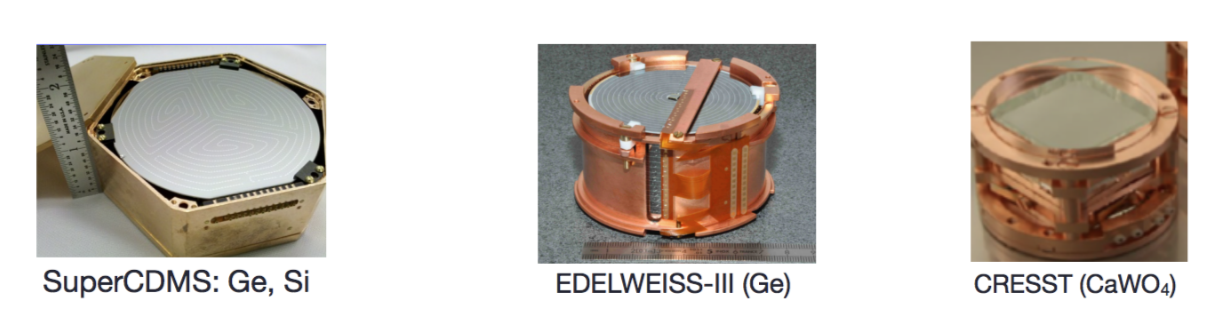
\includegraphics[scale=0.5]{figs/bolometerdetector.png}
%\begin{itemize}
%\item I bolometri usano cristalli raffreddati ($T \sim mK$)
%\item Ogni volta che una particella interagisce con il cristallo,
 % rilascia nel cristallo una certa quantit\`a di energia 
%\item Questa energia causa un aumento della temperatura del cristallo
%  che viene misurata con termometri a transizione di fase
%  superconduttiva (tungsteno)
%\item Si tratta di un aumento di temperatura di qualche
%  decina/centinaia di $\mu K$ per MeV
%\end{itemize}
\end{column}
\end{columns}
}

\frame{\frametitle{Ricerche DM dirette}
\begin{columns}[c]
\begin{column}{0.55\linewidth}
\centering
Stato attuale\\
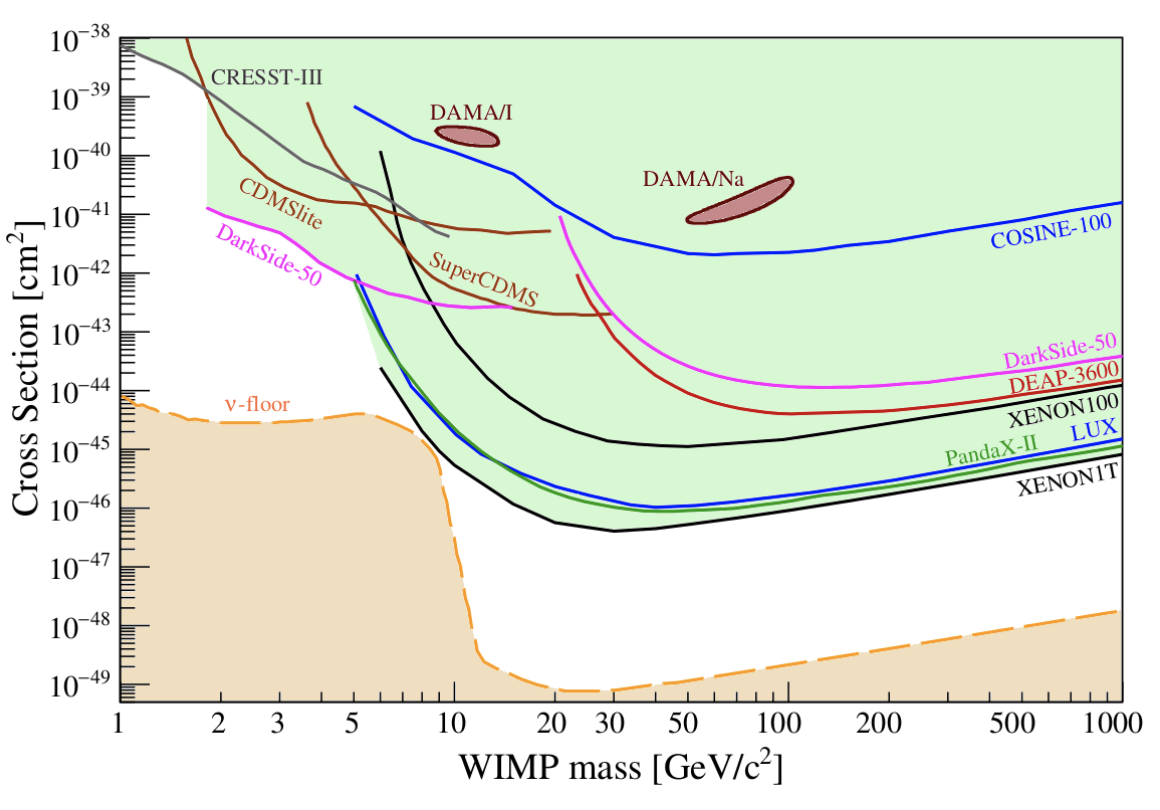
\includegraphics[scale=0.3]{figs/DMsearcheslimittoday.png}
\end{column}
\begin{column}{0.55\linewidth}
\centering
Futuro\\
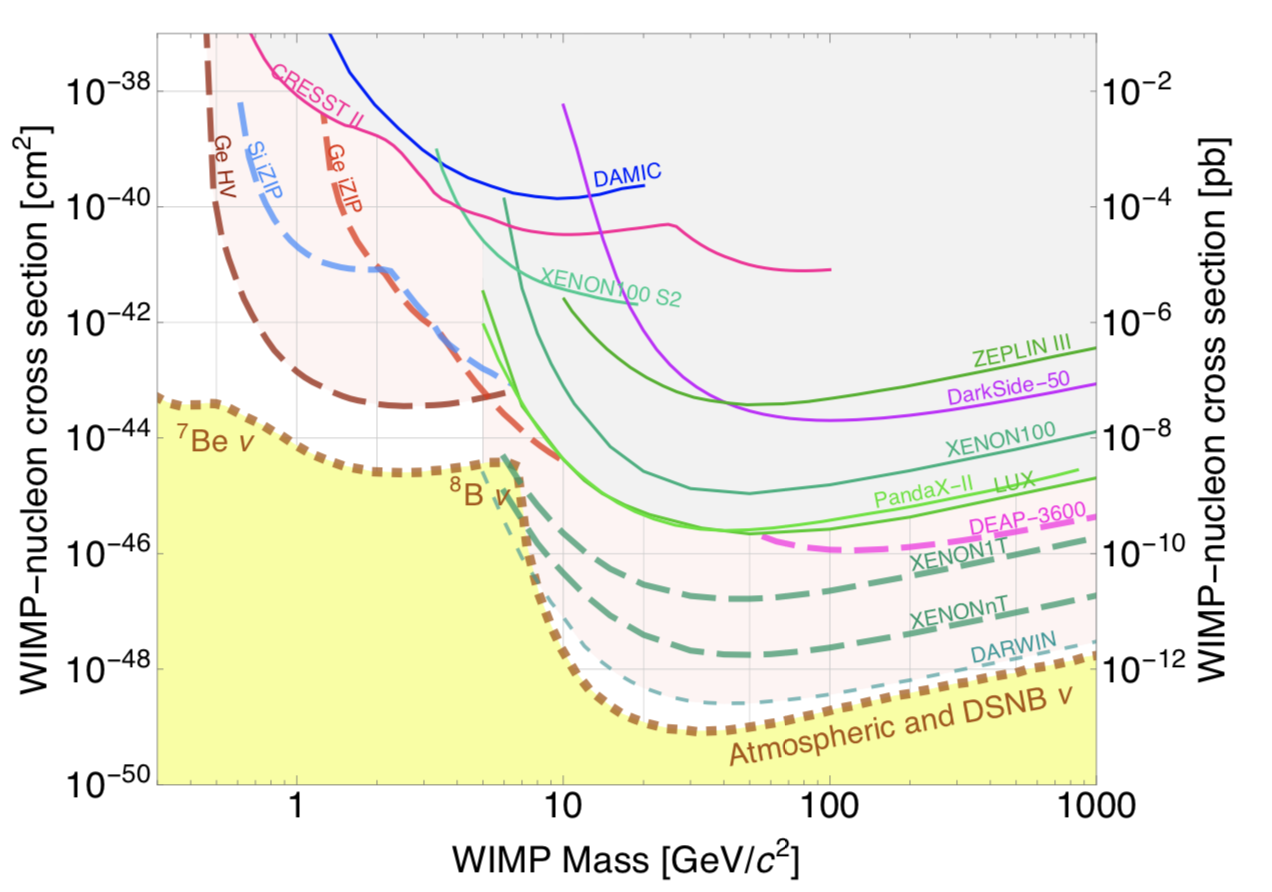
\includegraphics[scale=0.3]{figs/DMsearcheslimit.png}
\end{column}
\end{columns}
}


\frame{
\begin{itemize}
\item Per ora, nessuna evidenza di DM n\`e diretta, indiretta o ai collider
\item Ma moltissime nuove idee sulla natura della DM e nuovi settori da esplorare!
\end{itemize}
}


\frame{\frametitle{Neutrini: Dirac o Majorana?}
\vskip -0.3cm
\begin{columns}[c]
\begin{column}{1.0\linewidth}
\begin{itemize}
\scriptsize
\item Le masse dei neutrini sono molto diverse da quelle degli altri
  fermioni, perch\'e?
\end{itemize}
\centering
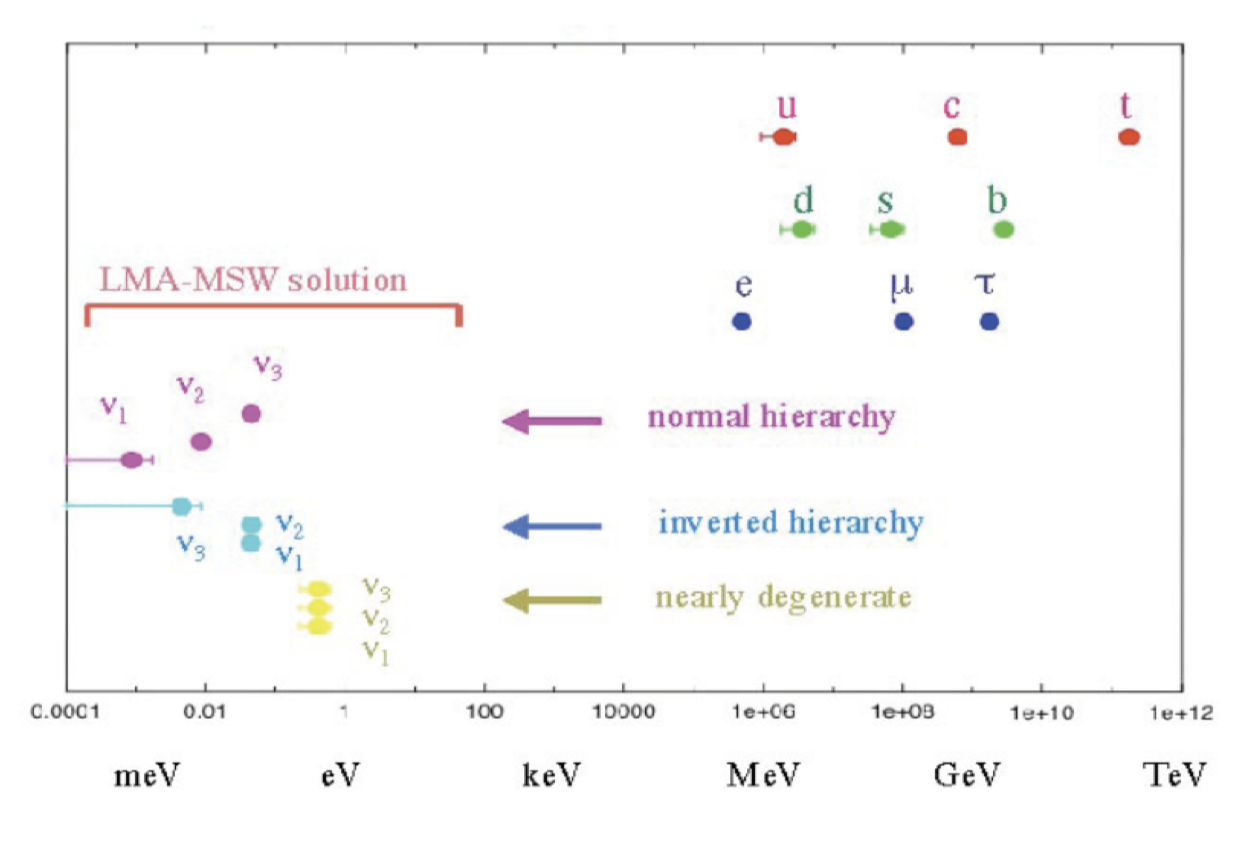
\includegraphics[scale=0.3]{figs/neutrinohierarchy.png}
\begin{itemize}
\scriptsize
\item Nel MS i neutrini sono senza massa (esiste un neutrino
  left-handed $\nu_{L}$ che si accoppia ai bosoni W Z )
\item Si possono includere le masse dei neutrini con lo stesso
  meccanismo di quelle dei fermioni
\item In generale, ci sono due possibili termini di massa per i
  fermioni: Dirac e di Majorana
\item Tutti i fermioni possono avere termini di messa di Dirac ma solo
  i fermioni neutri possono avere i termini di massa di Majorana
\end{itemize}
\end{column}
\end{columns}
}


\frame{\frametitle{Neutrini: Dirac o Majorana?}
\begin{columns}[c]
\begin{column}{1.0\linewidth}
\vskip -0.3cm
\begin{itemize}
\scriptsize
\item L'interazione gauge-invariante di Higgs con i fermioni fornisce
  i termini di Yukawa\\
$L_{massa} = -m_{D}\bar{\psi}_{L}\psi_{R} +
  h.c. = -m_{D} (\bar{\nu}_{L}\nu_{R} + h.c.)$ 
  con $m_{D} = \lambda \frac{v}{\sqrt{2}}$ dove $\lambda$ sono gli
  accoppiamenti di Yukawa
\item Nonostante sia possibile introdurre le masse di Dirac per i
  neutrini nel MS, la possibilit\`a di avere un termine di massa di
  Dirac \`e poco plausibile a causa del fatto che per avere masse
  molto piccole, gli accoppiamenti di Yukawa al campo di Higgs
  dovrebbero essere innaturalmente piccoli
\item I valori assoluti delle masse dei neutrini sono sconosciuti ma
  da considerazioni cosmologiche e da misure di oscillazioni per il
  neutrino a massa pi\`u grande\\
$5 \times 10^{-2} \unitm{eV} \sim (\sqrt{\Delta m^{2}_{A}}) \leq
m_{3} \leq \frac{1}{3}(\sum_{i=1}^{3}) \sim 0.3
\unitm{eV}$\\
dove $\Delta m^{2}_{A}$
 \`e la differenza di massa quadrata per il neutrino atmosferico\\
da cui: $2 \times 10^{-13} \leq \lambda^{\nu}_{3} \leq 10^{-12}$\\
da confrontare con gli accoppiamenti di altre particelle della terza
famiglia:\\
$\lambda_{t} \sim 7 \times 10^{-1}$, $\lambda_{b} \sim 2 \times
10^{-2}$, $\lambda_{\tau} \sim 7 \times 10^{-3}$\\
\item Per cui l'accoppiamento di Yukawa del neutrino pi\`u pesante \`e
  pi\`u di 10 ordini di grandezza pi\`u piccolo degli accoppiamenti delle altre
  particelle della terza famiglia
%\item In aggiunta, nella Lagrangiana del MS (che non include Yukawa)
%  entrano i campi sinistrorsi e distrorsi di tutte le particelle
%  cariche per cui la generazione delle masse non richiede gradi di
%  libert\`a aggiuntivi 
%\item Al contrario per il neutrino \`e sufficiente avere neutrini
%  sinistrorsi, per cui la generazione delle masse dei neutrini
%  richiede un neutrino destrorso e quindi un grado di libert\`a addizionale
\end{itemize}
\end{column}
\end{columns}
}

\frame{\frametitle{Neutrini: Dirac o Majorana?}
\begin{columns}[c]
\begin{column}{1.0\linewidth}
\begin{itemize}
\scriptsize
\item L'idea di base \`e quello di assumere l'esistenza solo di
  neutrini sinistrorsi: il termine di massa di Majorana include solo
  un campo che si accoppia con se stesso 
\item Consideriamo l'operazione di coniugazione di carica:\\
$\nu^{c}_{L} = C\bar{\nu}_{L}^{T}$ dove C \`e la matrice di
coniugazione di carica $C\gamma_{\mu}^{T} C^{-1} = -\gamma_{\mu}$
\item $\nu^{c}_{L} = \nu_{R}$ \`e destrorso
\item Il campo di Majorana \`e dato da $\nu = \nu_{L} + \nu_{R}
  =\nu_{L} + \nu^{c}_{L}$:\\ $\nu = \nu^{c}$ i neutrini sono la loro
  stessa antiparticella (cio\`e un neutrino di Majorana \`e lo stesso
  di un anti-neutrino di Majorana)
\item Per cui \`e possibile scrivere il termine di massa di
  Majorana:\\
$L^{M} =
-\frac{m}{2}(\bar{\nu}^{c}_{L}\nu_{L}+\bar{\nu}_{L}\nu_{L}^{c})$ 
\item poich\`e $\nu_{L}$ ha $L=+1$ e $\nu^{c}_{L}$ ha $L =-1$: il
  numero leptonico totale non \`e conservato $\Delta L = \pm 2$
%\item Nella rappresentazione chirale ho solo due gradi di libert\`a
\end{itemize}
\centering
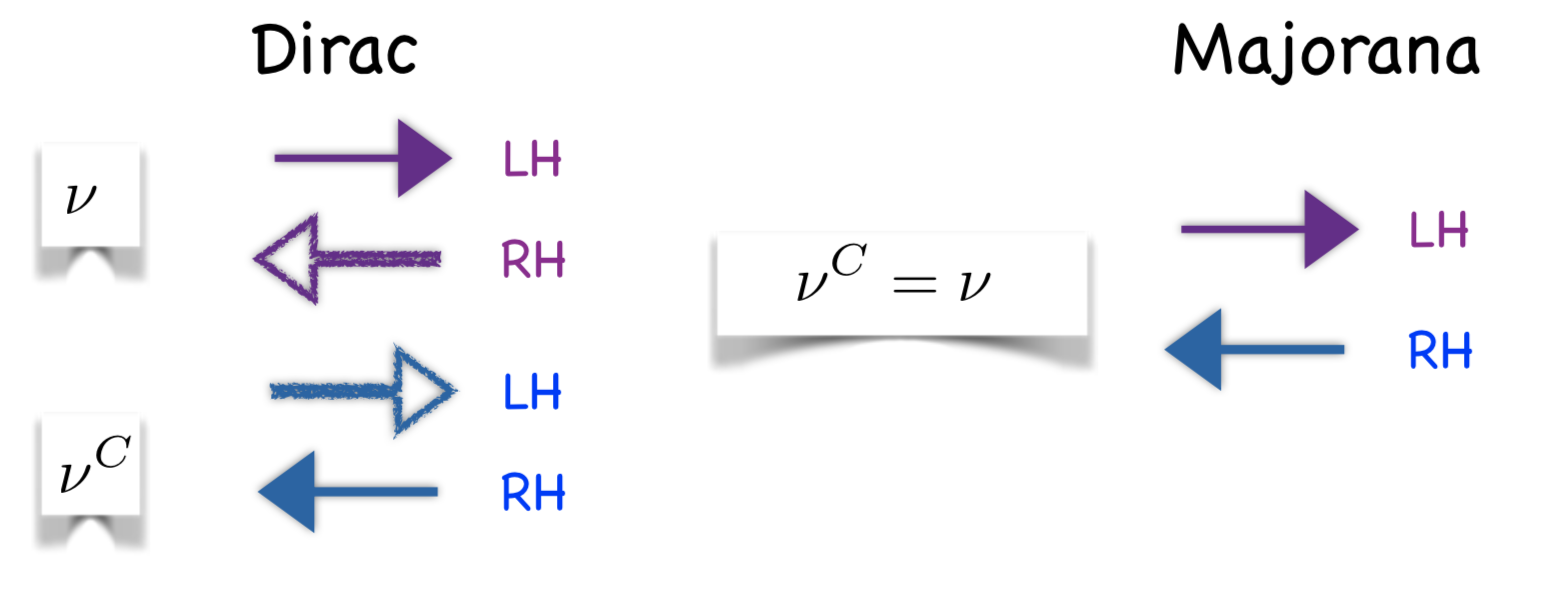
\includegraphics[scale=0.2]{figs/diracmajorana.png}
\end{column}
\end{columns}
}

\frame{\frametitle{}
\begin{columns}[c]
\begin{column}{1.0\linewidth}
\begin{itemize}
\scriptsize
\item Gli effetti di rimuovere la distinzione tra neutrini e
  anti-neutrini sono molto piccoli
\item Il neutrino prodotto dal decadimento $\pi^{+} \to
  \mu^{+}\nu_{\mu}$ produce un $\mu^{-}$ nell'interazione di corrente
  carica $\nu_{\mu}n \to \mu^{-}p$
\item Per cui il numero leptonico L = N(leptoni)-N(antileptoni) \`e
  costante (conservato) nel Modello Standard
\item Se invece $\nu_{\mu}$ fosse un neutrino di Majorana potrebbe
  interagire come antiparticella destrorsa $\nu_{M}p \to \mu^{+} n$
\item Questo implicherebbe la non-conservazione del numero leptonico
  $\Delta L = -2$
\item Tuttavia, visto le piccole masse dei neutrini, gli stati di
  elicit\`a corrispondono circa agli stati chirali e i processi che
  violano il numero leptonico sarebbero soppressi ${\mathcal
    O}(m^{2}_{\nu}/m^{2}_{\mu})$ (troppo piccolo per essere
  osservabile)
\item Sperimentalmente si cercano decadimenti doppio-beta senza
  neutrini che possono avvenire solo se i neutrini sono particelle di Majorana
\end{itemize}
\end{column}
\end{columns}

}


\frame{\frametitle{Ricerca di decadimenti $0\nu\beta\beta$}
\begin{columns}[c]
\begin{column}{0.6\linewidth}
\begin{itemize}
\scriptsize
\item Il decadimento doppio $\beta$ \`e un processo raro al secondo
  ordine che pu\`o essere pensato come due decadimenti $\beta$
  simultanei con l'emissione di due elettroni da un nucleo
\item Insieme ai due elettroni, vengono emessi due anti-neutrino
\item Decadimenti $2\nu\beta\beta$ sono rari con vite medie
  $\tau=10^{19}$-$10^{25}$ anni 
\item Prima osservazione nel 1987, oggi osservati nel decadimento di
  diversi isotopi
\item Se i neutrini sono particelle di Majorana \`e possibile avere processi di
  decadimenti doppio-beta senza neutrini che violano il numero
  leptonico $\Delta L =2 $

\end{itemize}
\end{column}
\begin{column}{0.55\linewidth}
\centering
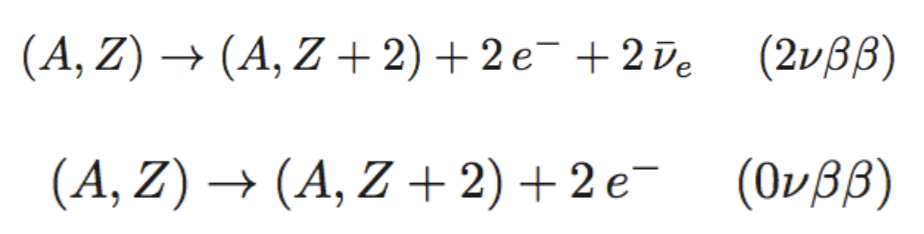
\includegraphics[scale=0.3]{figs/neutrinolessequation.png}\\
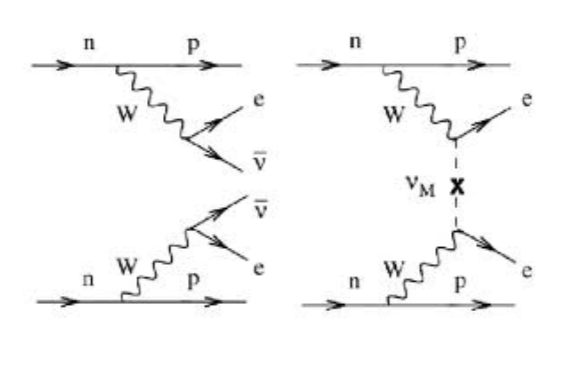
\includegraphics[scale=0.5]{figs/decayneutrinoless.png}
\end{column}
\end{columns}
}

\frame{\frametitle{Esperimenti $0\nu\beta\beta$: strategia}
\vskip -0.3cm
\begin{columns}[T]
\begin{column}{0.55\linewidth}
\begin{itemize}
\scriptsize
\item Sperimentalmente \`e possibile distinguere processi
  $0\nu\beta\beta$ da processi $2\nu\beta\beta$ dallo spettro degli
  elettroni: $0\nu\beta\beta$ producono elettroni mono-energetici\\
$E_{e} = \frac{1}{2}(M(Z,A)-M(Z+2,A))$\\
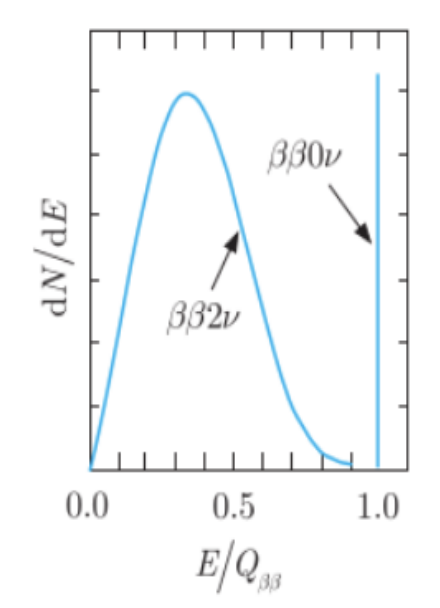
\includegraphics[scale=0.35]{figs/spettrodopppiobeta.png}
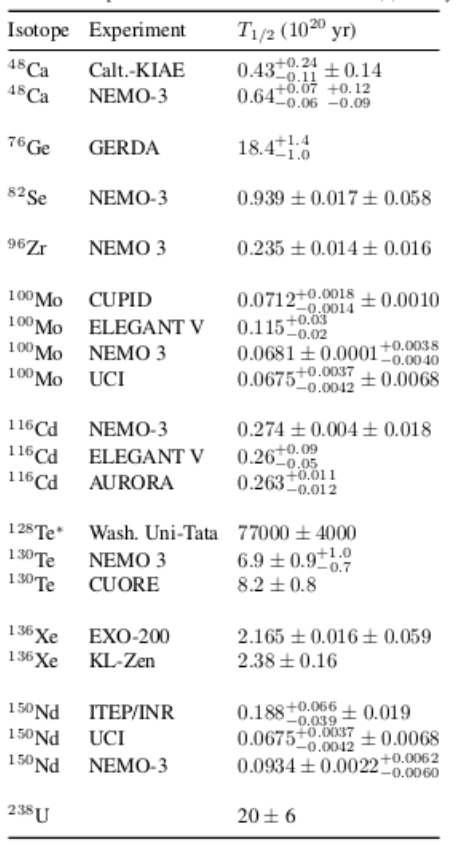
\includegraphics[scale=0.35]{figs/isotopidoppiobeta.png}
\end{itemize}
\end{column}
\begin{column}{0.55\linewidth}
\begin{itemize}
\scriptsize
\item Diversi nuclei per lo studio di
  $0\nu\beta\beta$
\begin{itemize}
\scriptsize
\item Alto Q-value (rigetta la maggior parte della radioattivit\`a
  naturale)
\item Elevato numero di nuclei: tenere conto dell'abbondanza naturale
  dell'isotopo, possibile arricchimento ma costoso (${}^{130}Te$ elevata abbondanza naturale)  
\end{itemize}
\scriptsize
\item Rivelatori
\begin{itemize}
\scriptsize
\item Elevata risoluzione energetica per ridurre il fondo da $2\nu\beta\beta$: linea monocromatica al Q-value
  del decadimento 
\item Basso fondo: esperimenti sotterranei, purificazione del
  materiale degli esperimenti
\end{itemize}
\scriptsize
\item Diverse tecniche di rivelazione (Bolometri, Semiconduttori,
  Scintillatori Liquidi, TPC, ...)
\end{itemize}
\end{column}
\end{columns}
\begin{columns}[T]
\begin{column}{1.15\linewidth}
\begin{itemize}
\scriptsize
\item Fino ad ora nessuna osservazione, limiti $\sim
  10^{26}$ anni (prossima generazione $\sim
  10^{28}$)
\end{itemize}
\end{column}
\end{columns}
}


\frame{
  \frametitle{Altri corsi legati a particelle}

  \begin{itemize}
  \item {\it TEORIA DELLE INTERAZIONI FONDAMENTALI}:\\ Modello Standard (settore elettrodebole).
  \item {\it FISICA DELLE INTERAZIONI FONDAMENTALI AI COLLIDER}:\\ Tecniche sperimentali per fisica delle particelle ai collider.
  \item {\it FISICA DELLE ASTROPARTICELLE}: \\ Tecniche sperimentali
    per fisica delle astroparticelle.
 \item {\it FISICA DEI RIVELATORI DI PARTICELLE}:\\ Interazione particelle materia. Rivelatori di particelle. 
  \item {\it LABORATORIO DI FISICA DELLE INTERAZIONI FONDAMENTALI E ASTROFISICA}:\\Interazione particelle materia. Rivelatori di particelle. Esperienze di laboratorio.
  \end{itemize}
}


